\section{Experimental Evaluation}

\begin{figure*}%figure 6
    \centering
    \subfloat[Running time comparison with various data sets.]{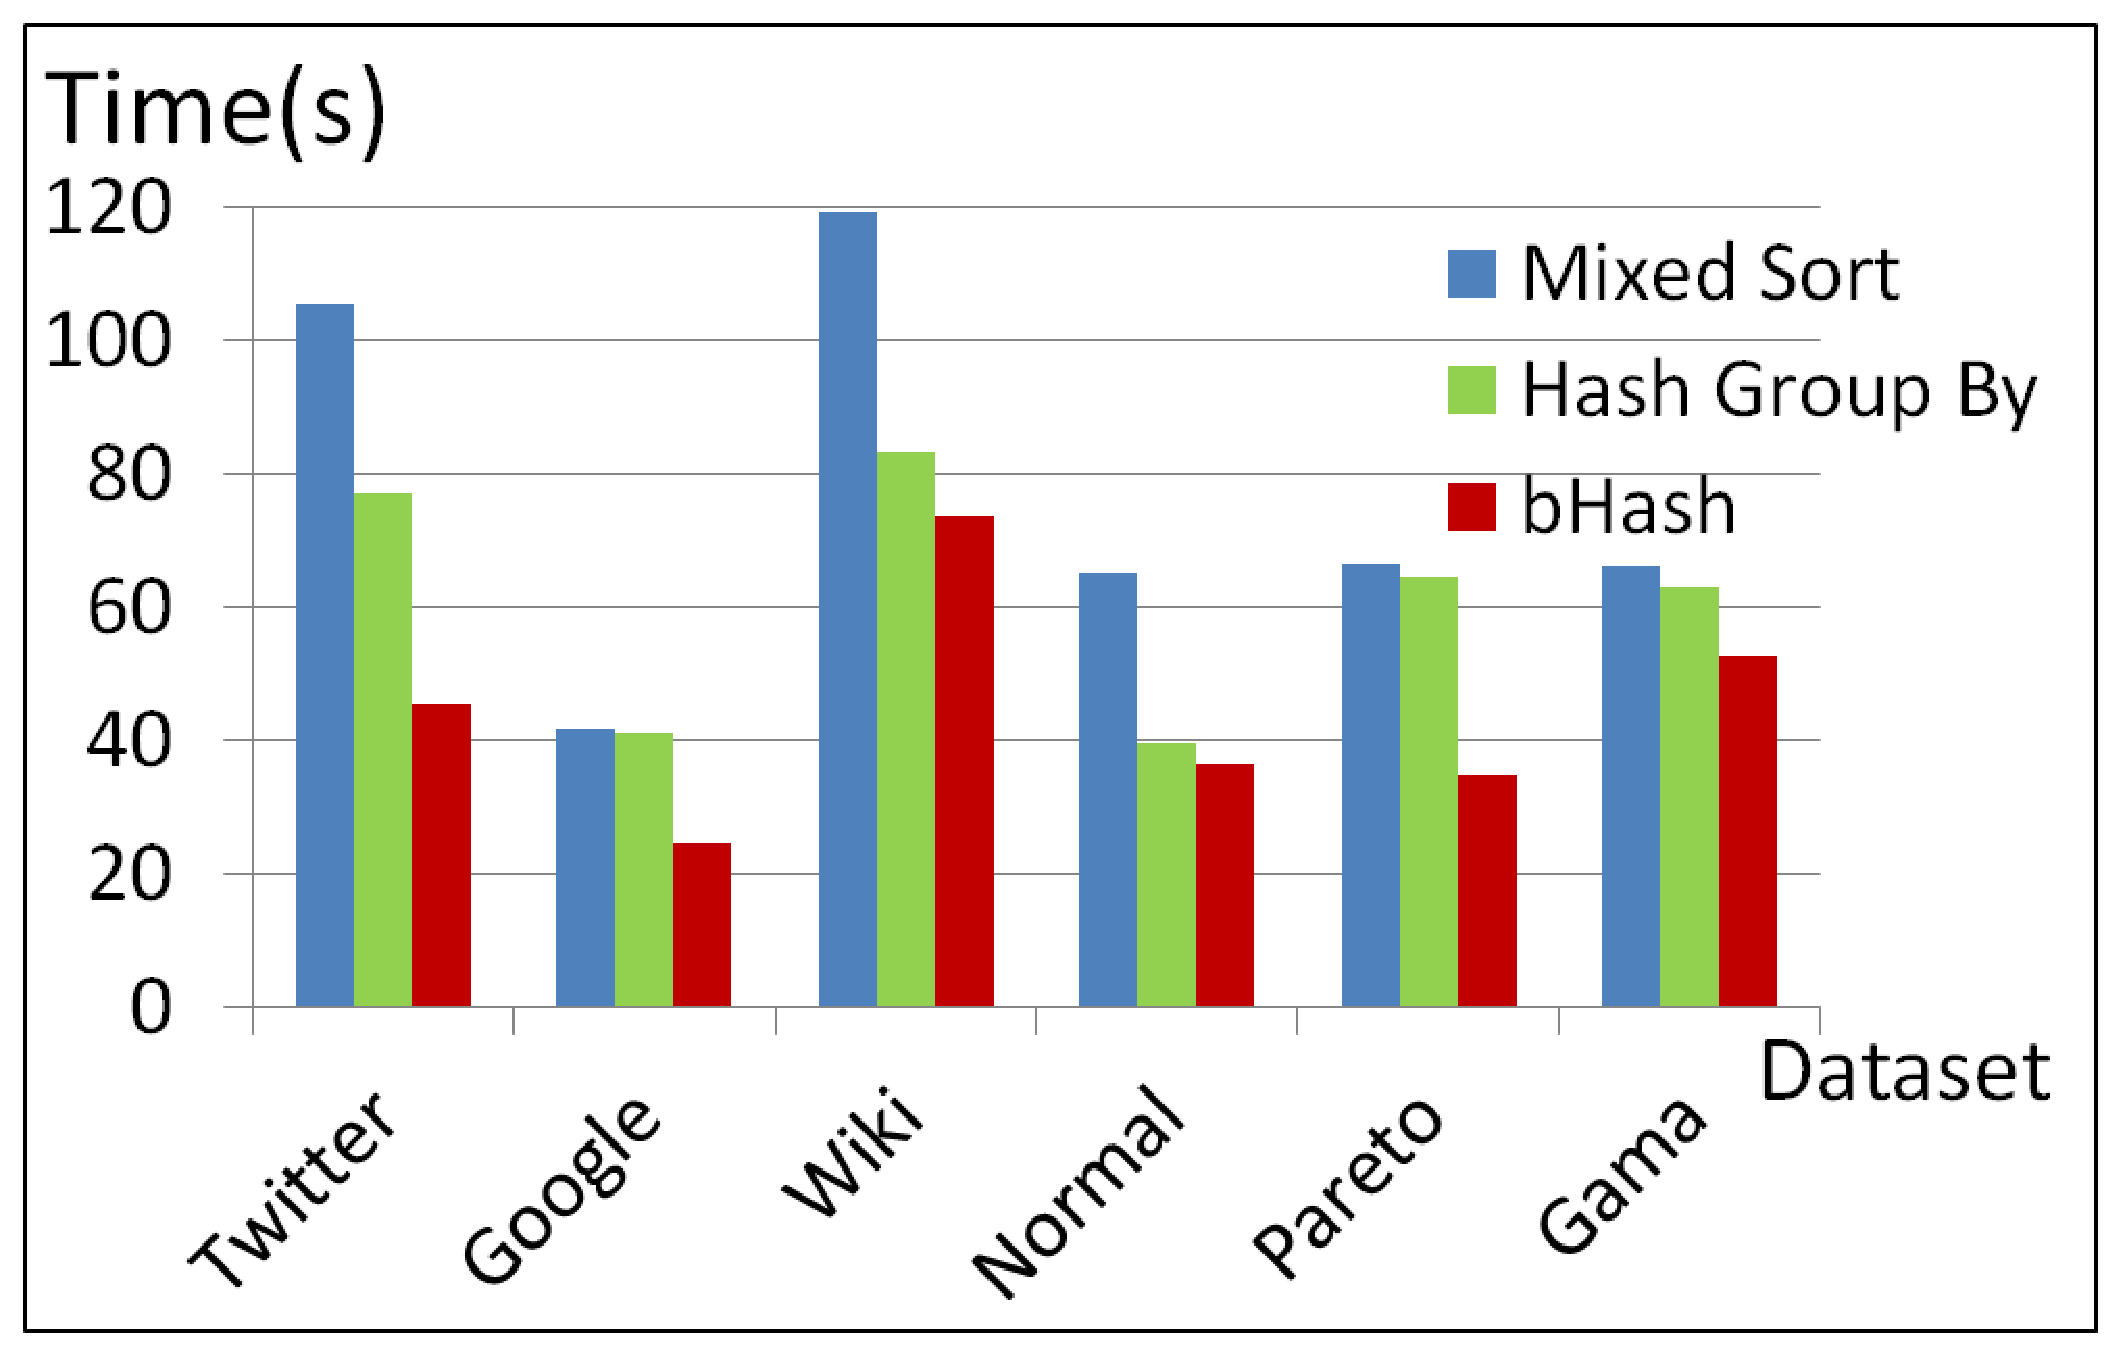
\includegraphics[width = 2in]{fig/datasetTime.eps}\label{fig:datasetTime}}\ \
    \hspace{1pt}
    \subfloat[Acceleration percentage compared with merge-sort]{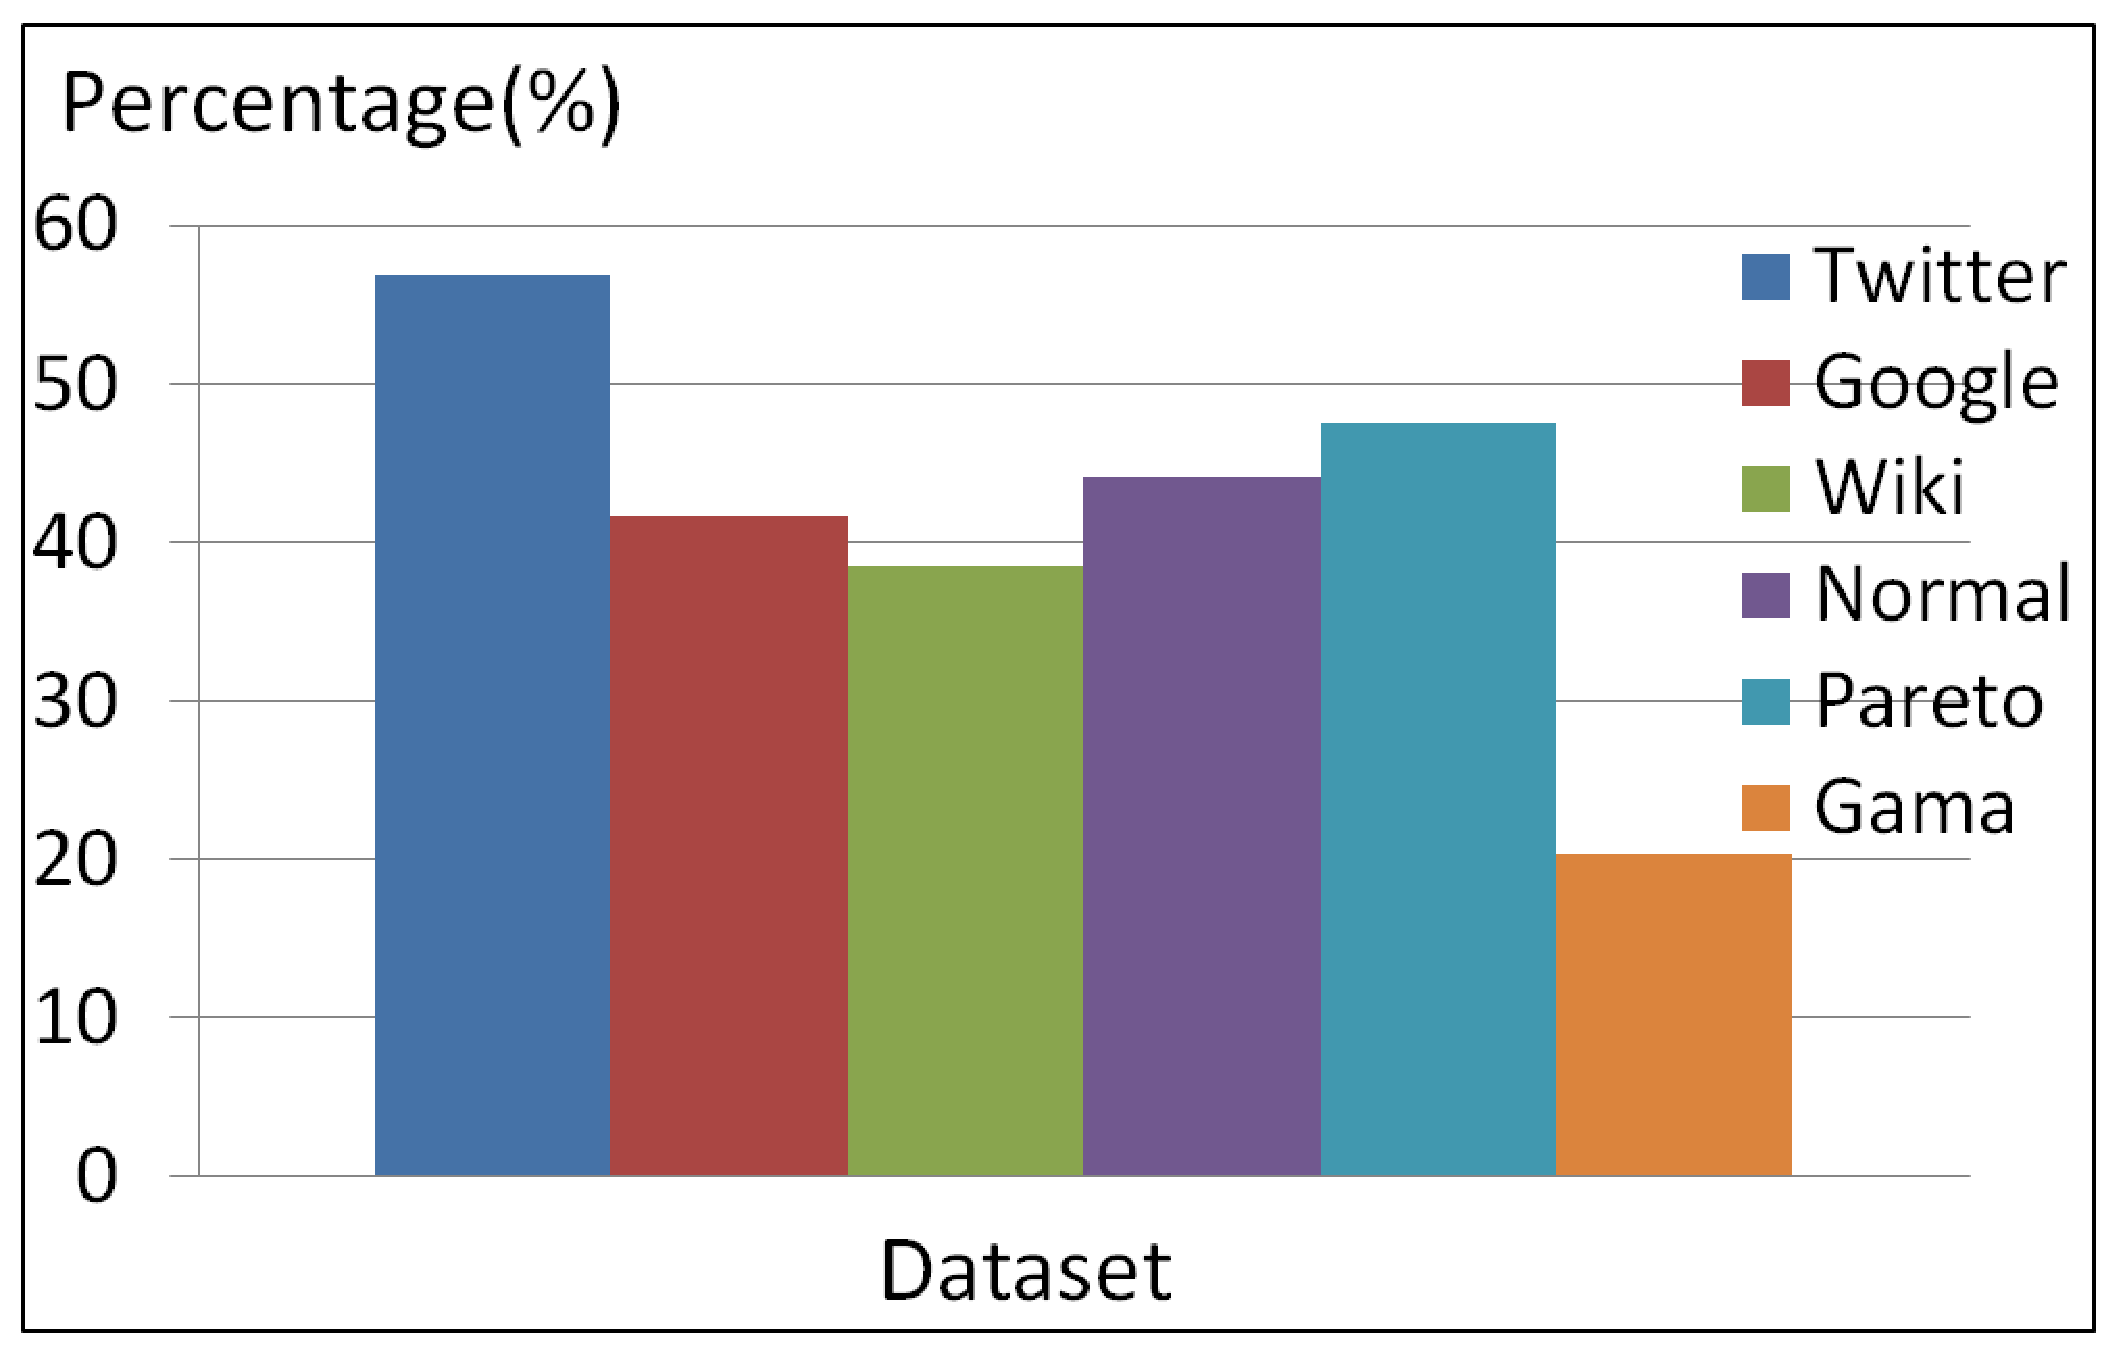
\includegraphics[width = 2in]{fig/percentageComparedSort.eps}\label{fig:percentageComparedSort}}\ \
    \hspace{1pt}
    \subfloat[Acceleration percentage compared with memory-constraint hash]{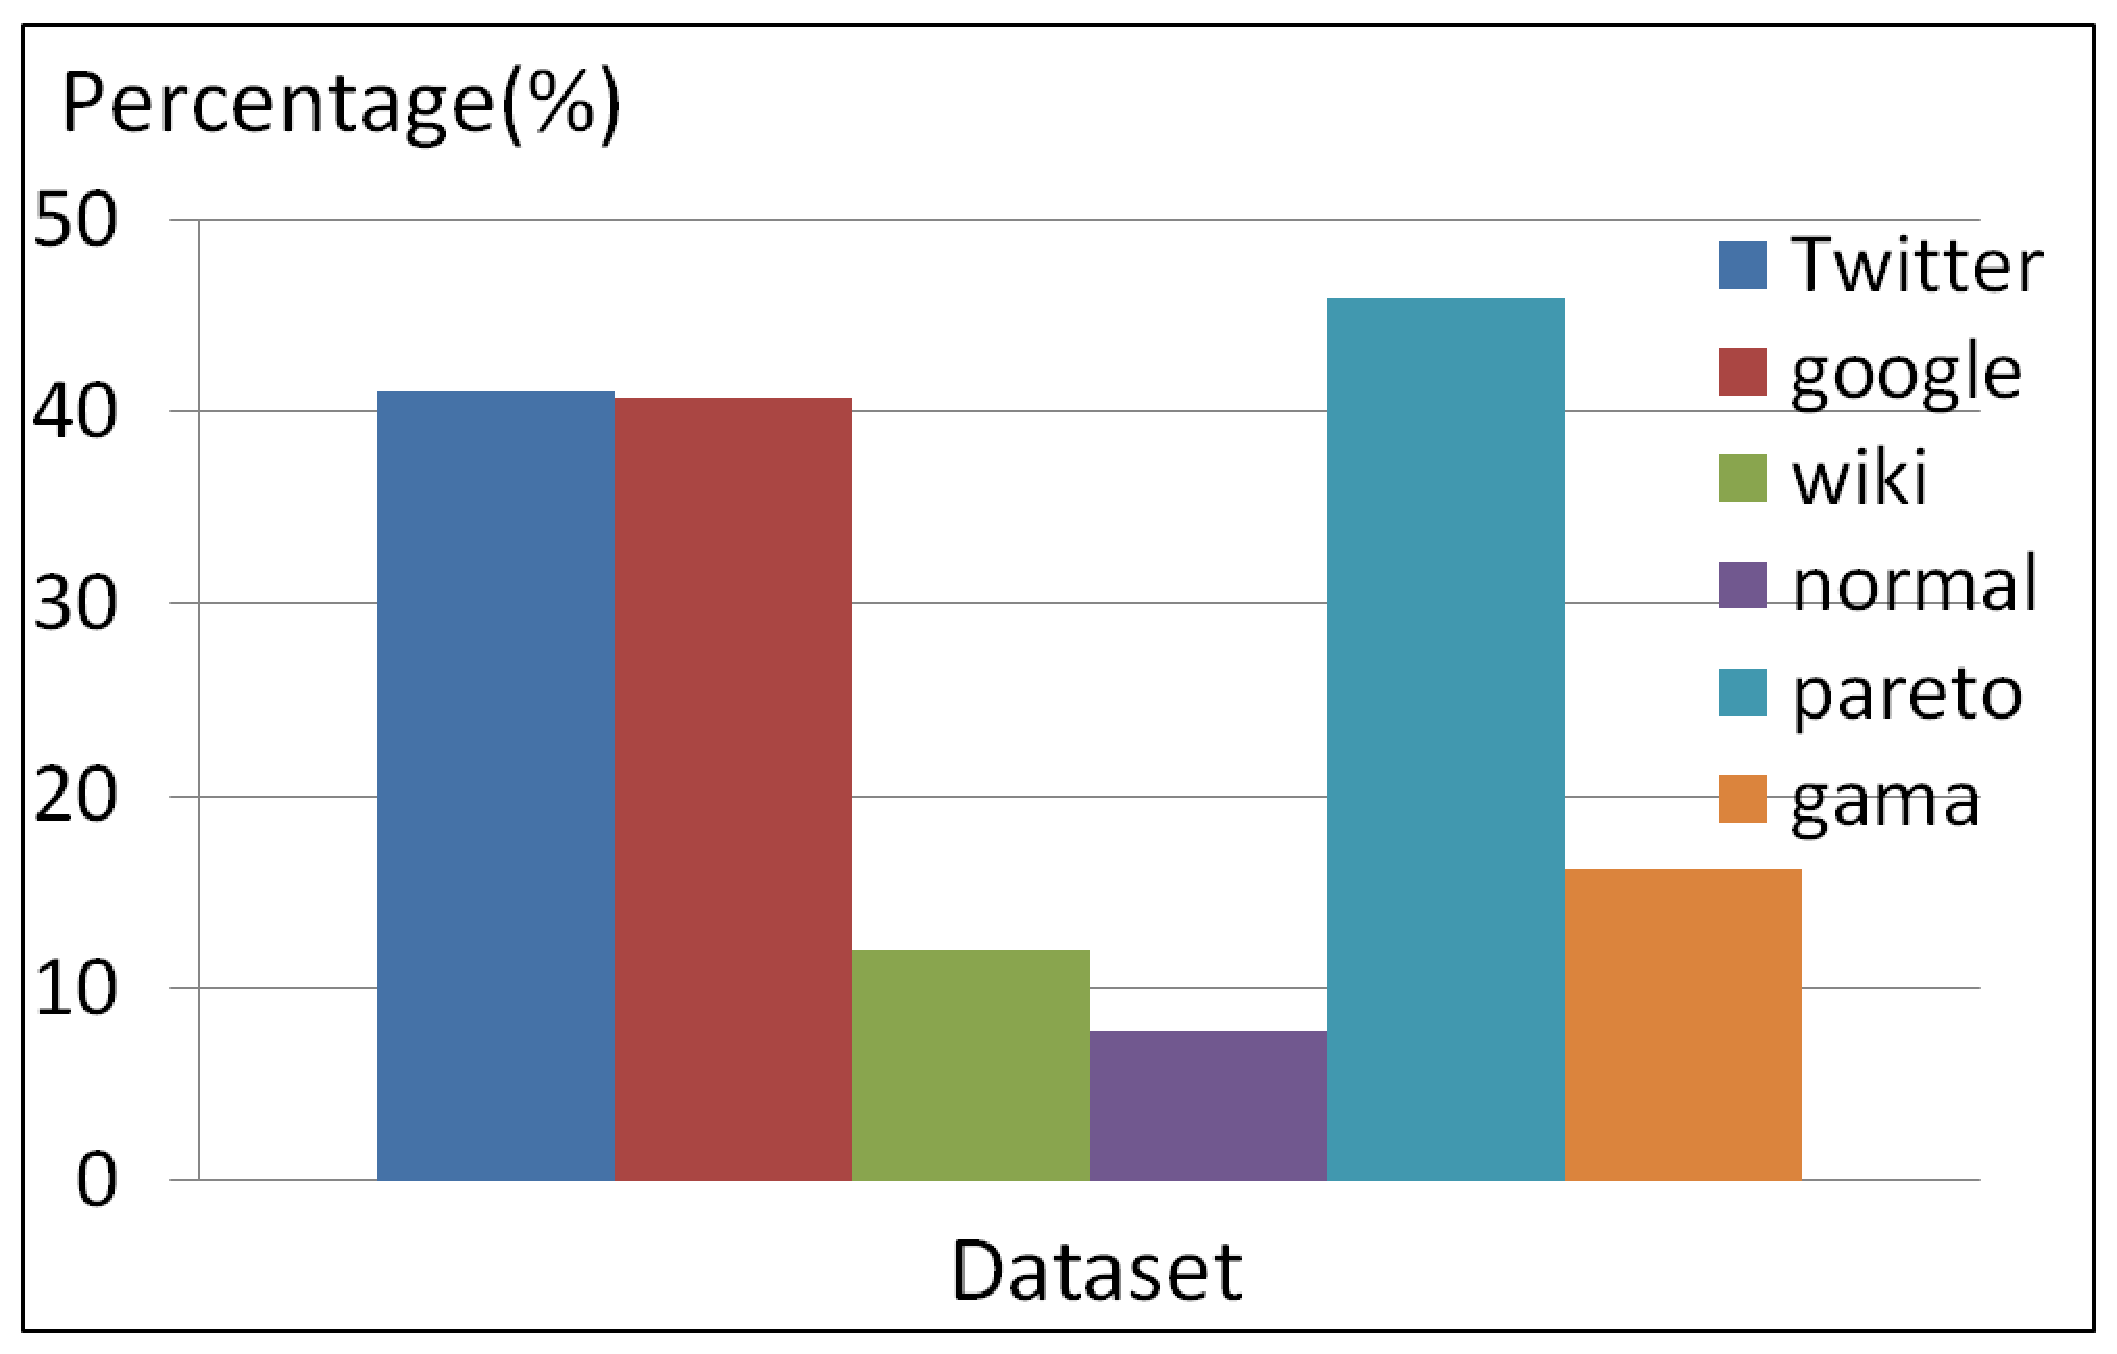
\includegraphics[width = 2in]{fig/percentageComparedHashGroupBy.eps}\label{fig:ComparedHashGroupBy}}\ \
    \caption{Running time and acceleration percentage under the same memory usage.}\label{fig:Running time and acceleration}
\end{figure*}

This section presents the performance evaluation for bHash. We compare our work against existing typical grouping approaches, merge-sort \cite{dean2008mapreduce} and memory-constraint hash \cite{bartholomew2012mariadb}. For merge-sort, we downloaded the implementation from the official sites. There is no source code for memory-constraint hash available, so we implemented our own hash aggregation version following the pseudo code in SQL database \cite{HashAggregate15}. We used typical real data sets:  (a) the Higgs\footnote{www.wikibench.eu/wiki/2007-09/wiki.1190153705.gz} Twitter data set, providing the information about activity on Twitter during the discovery of Higgs-boson; (b) the Google\footnote{http://snap.standford.edu/data/web-Google.txt.gz} web graph data set containing 870,000 nodes and 5,100,000 edges; (c) the Wiki\footnote{http://snap.standford.edu/data/higgs-twitter.html} data set containing 1.2GB different URLs; and three simulation data sets that obey different distributions including a Normal distribution and two weight-tailed distributions : Pareto and Gama. Table 1 summarizes the data sets used.

\begin{figure*}
    \centering
    \subfloat[Performance comparison on Wiki]{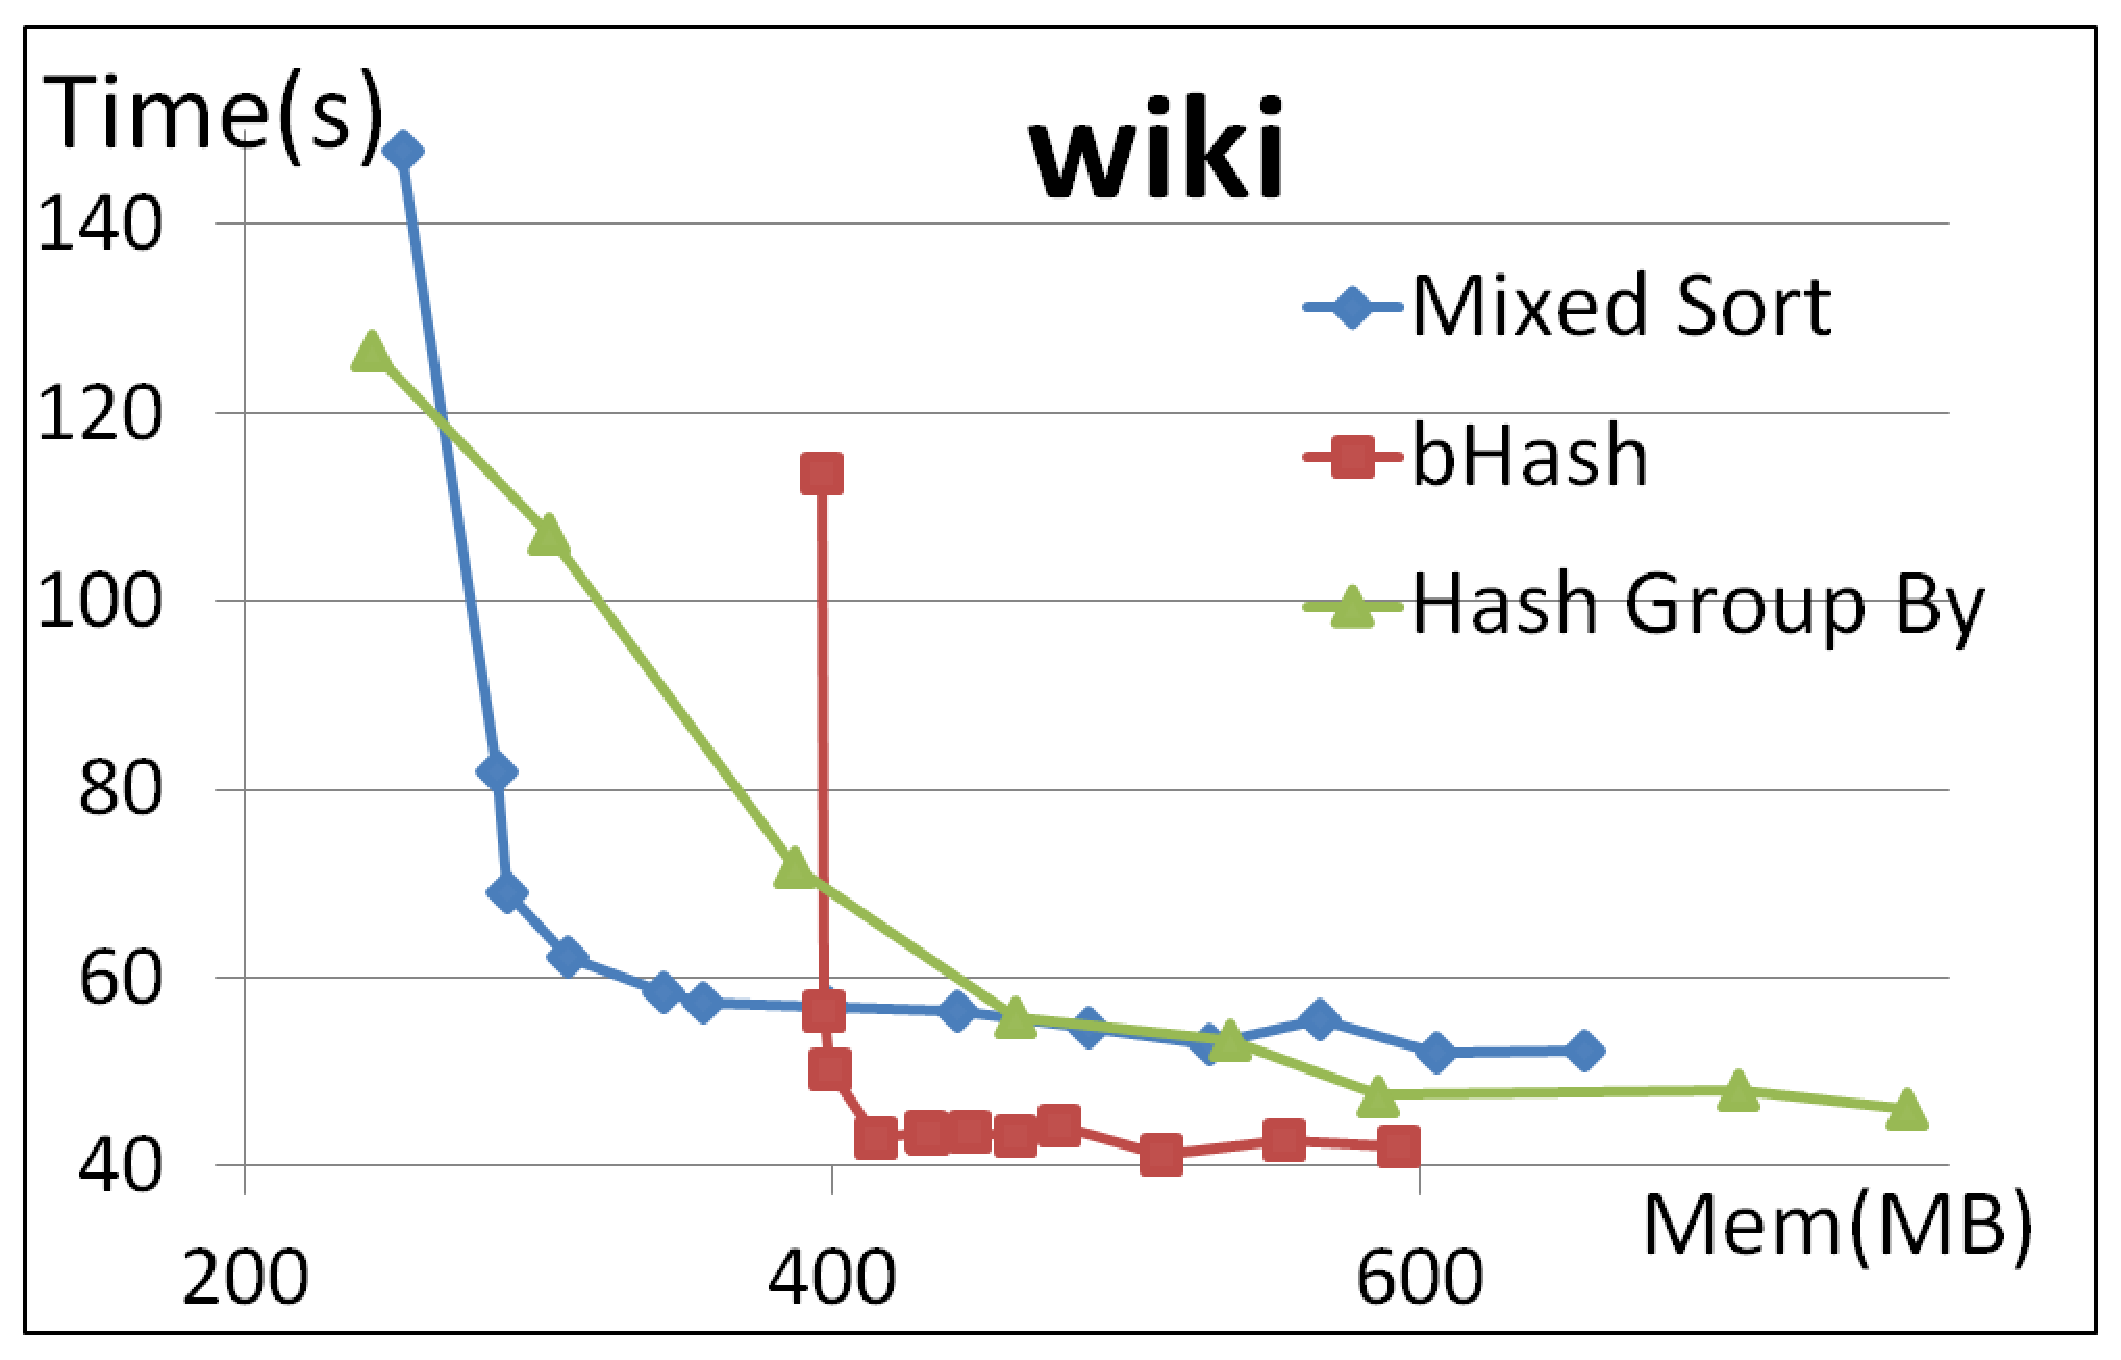
\includegraphics[width = 1.61in]{fig/wikiMemTime.eps}\label{fig:wikiMemTime}}\ \
    \hspace{0.5pt}
    \subfloat[Performance comparison on Twitter]{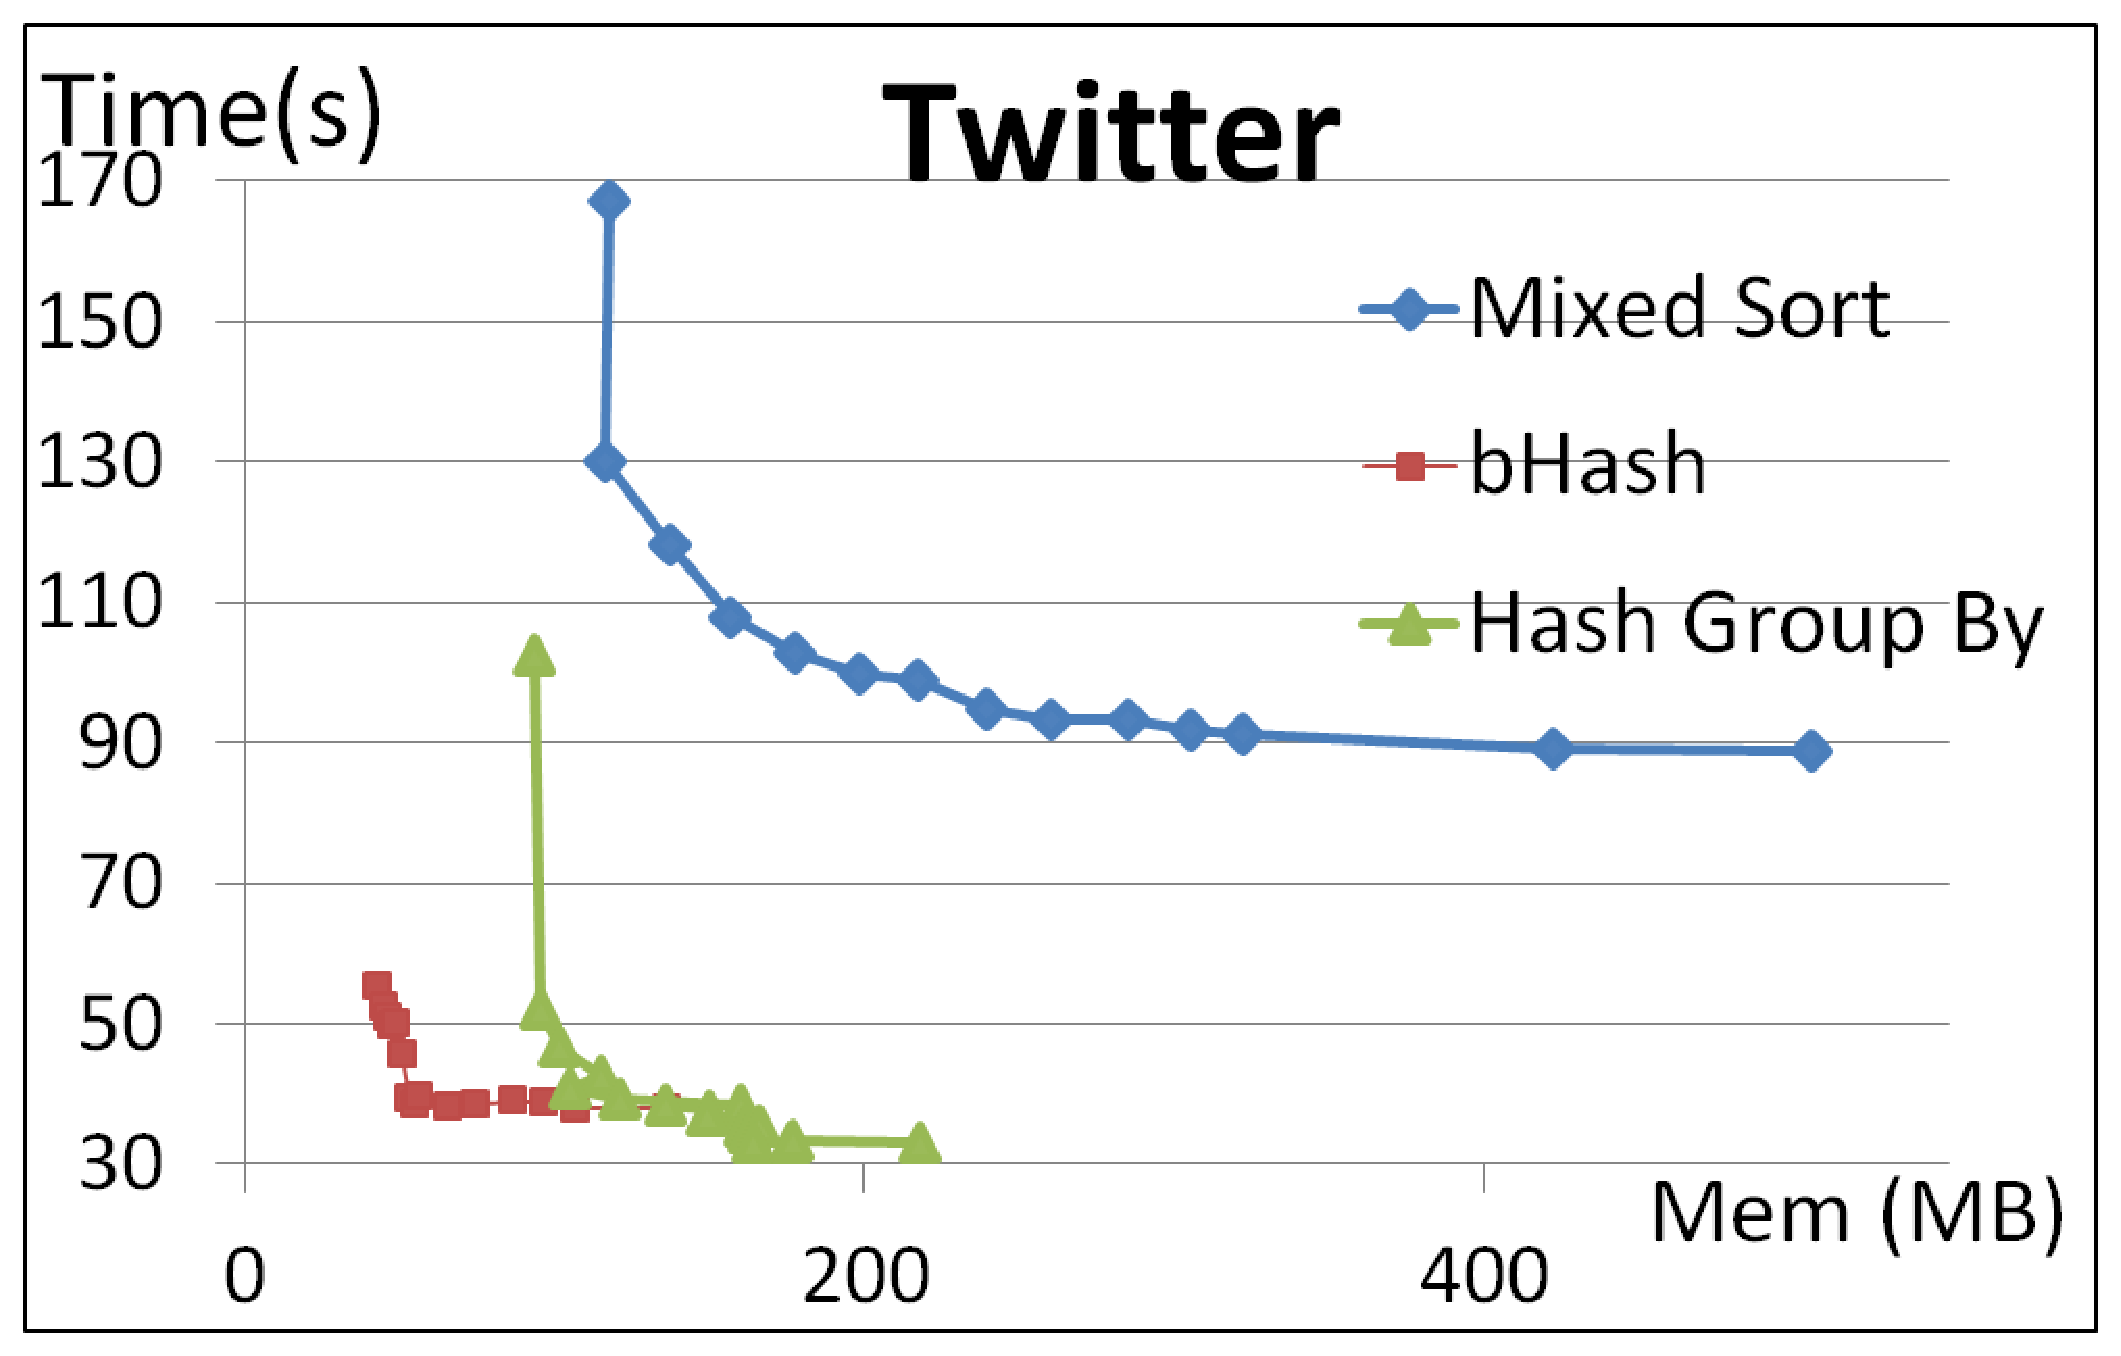
\includegraphics[width = 1.61in]{fig/twitterMemTime.eps}\label{fig:twitterMemTime}}\ \
   \hspace{0.5pt}
    \subfloat[Performance comparison on Normal]{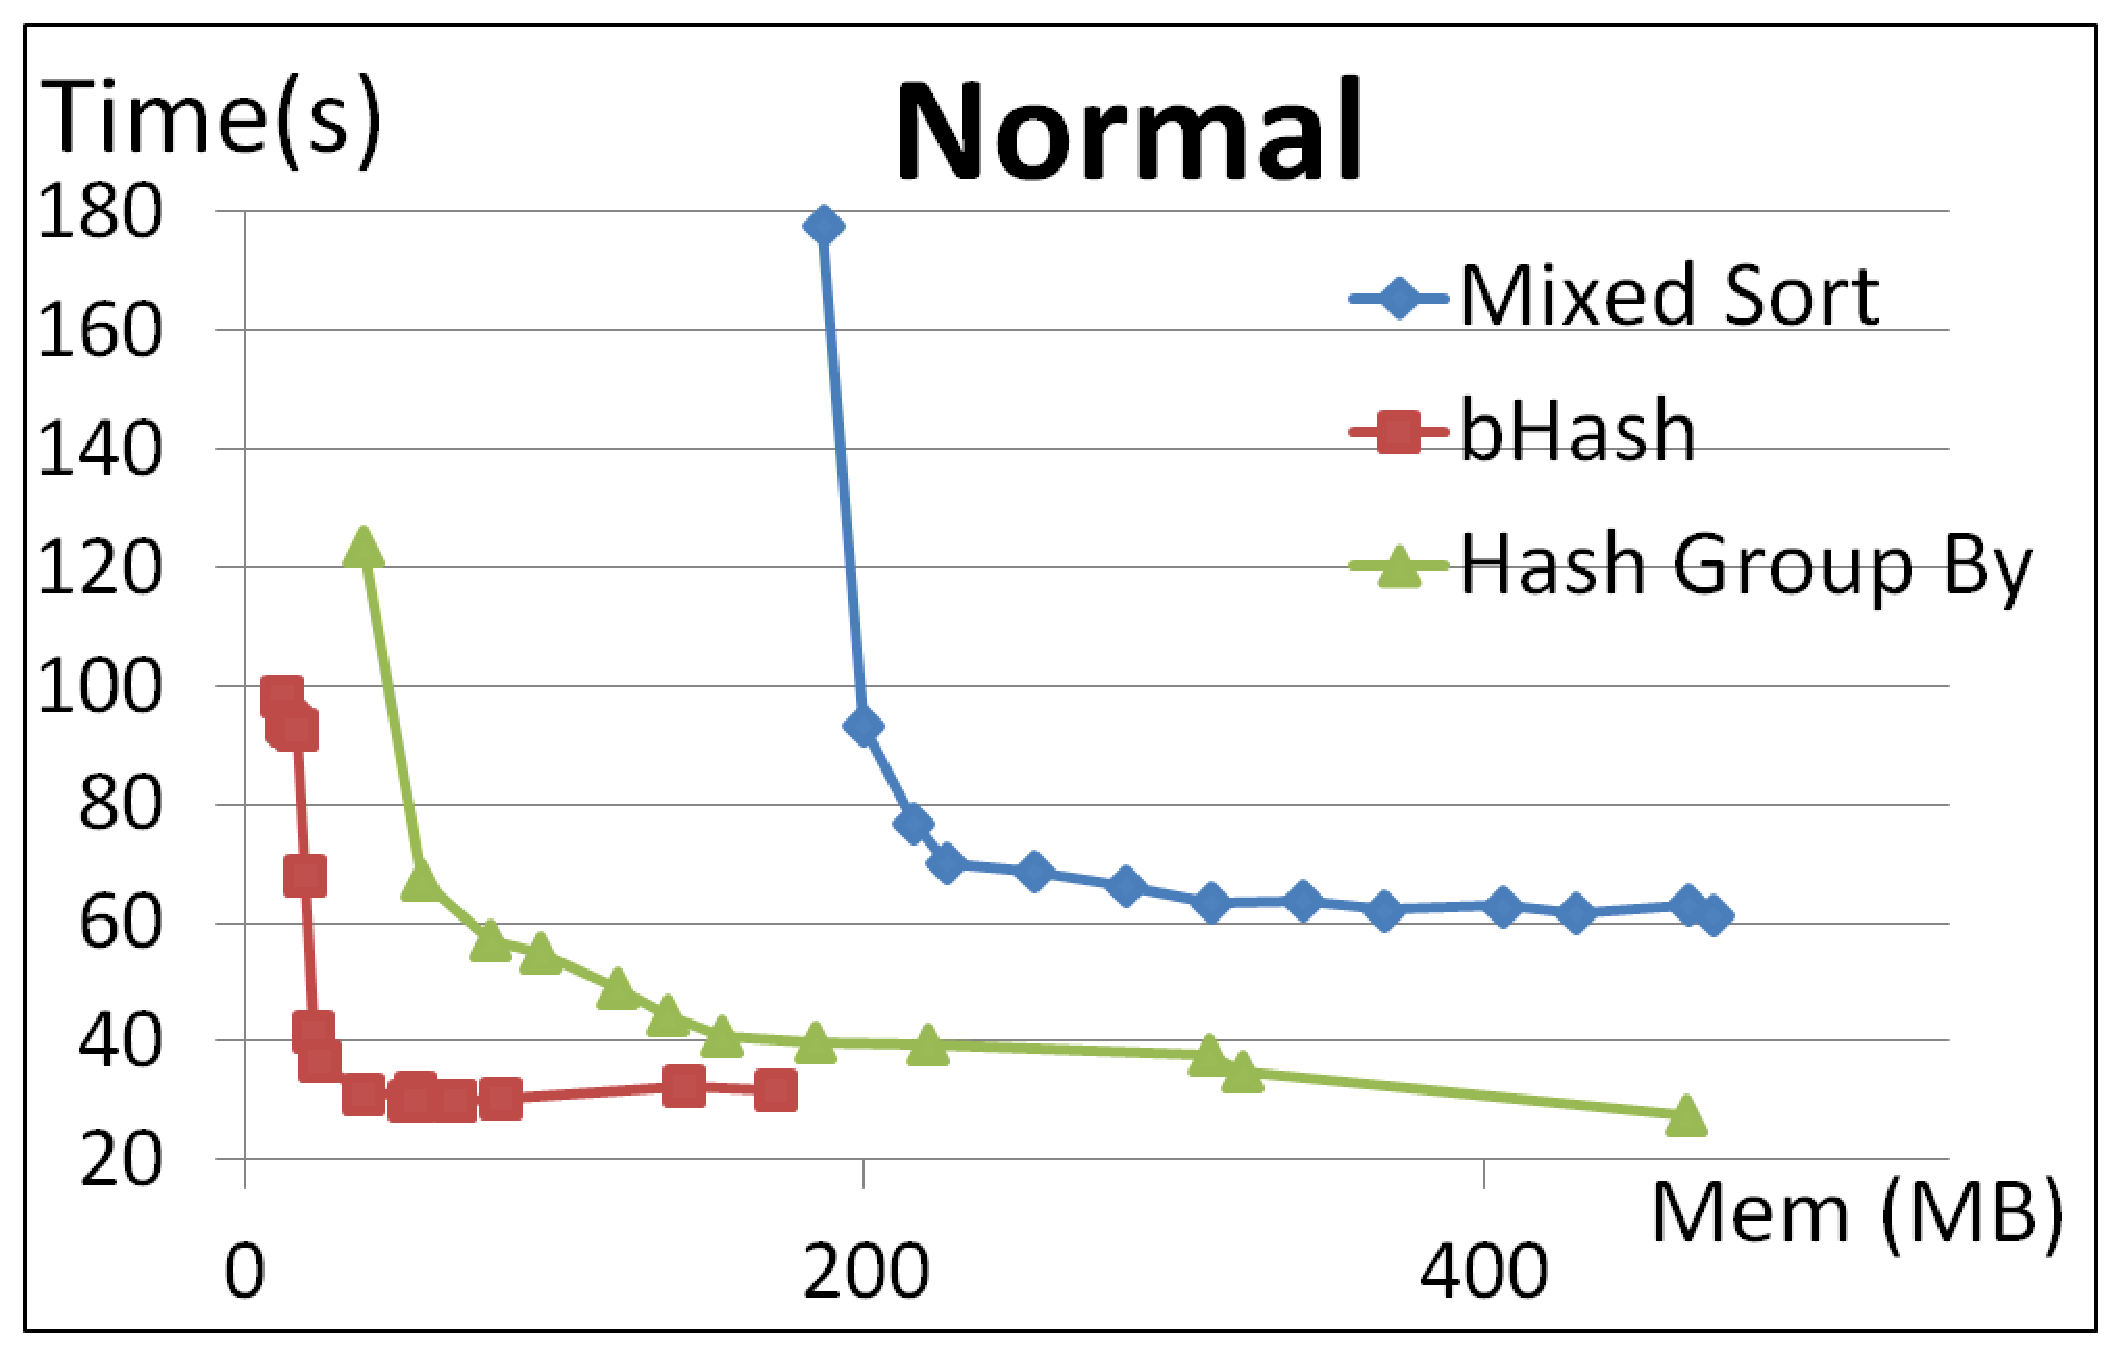
\includegraphics[width = 1.61in]{fig/normalMemTime.eps}\label{fig:normalMemTime}}\ \
     \hspace{0.5pt}
    \subfloat[Performance comparison on Pareto]{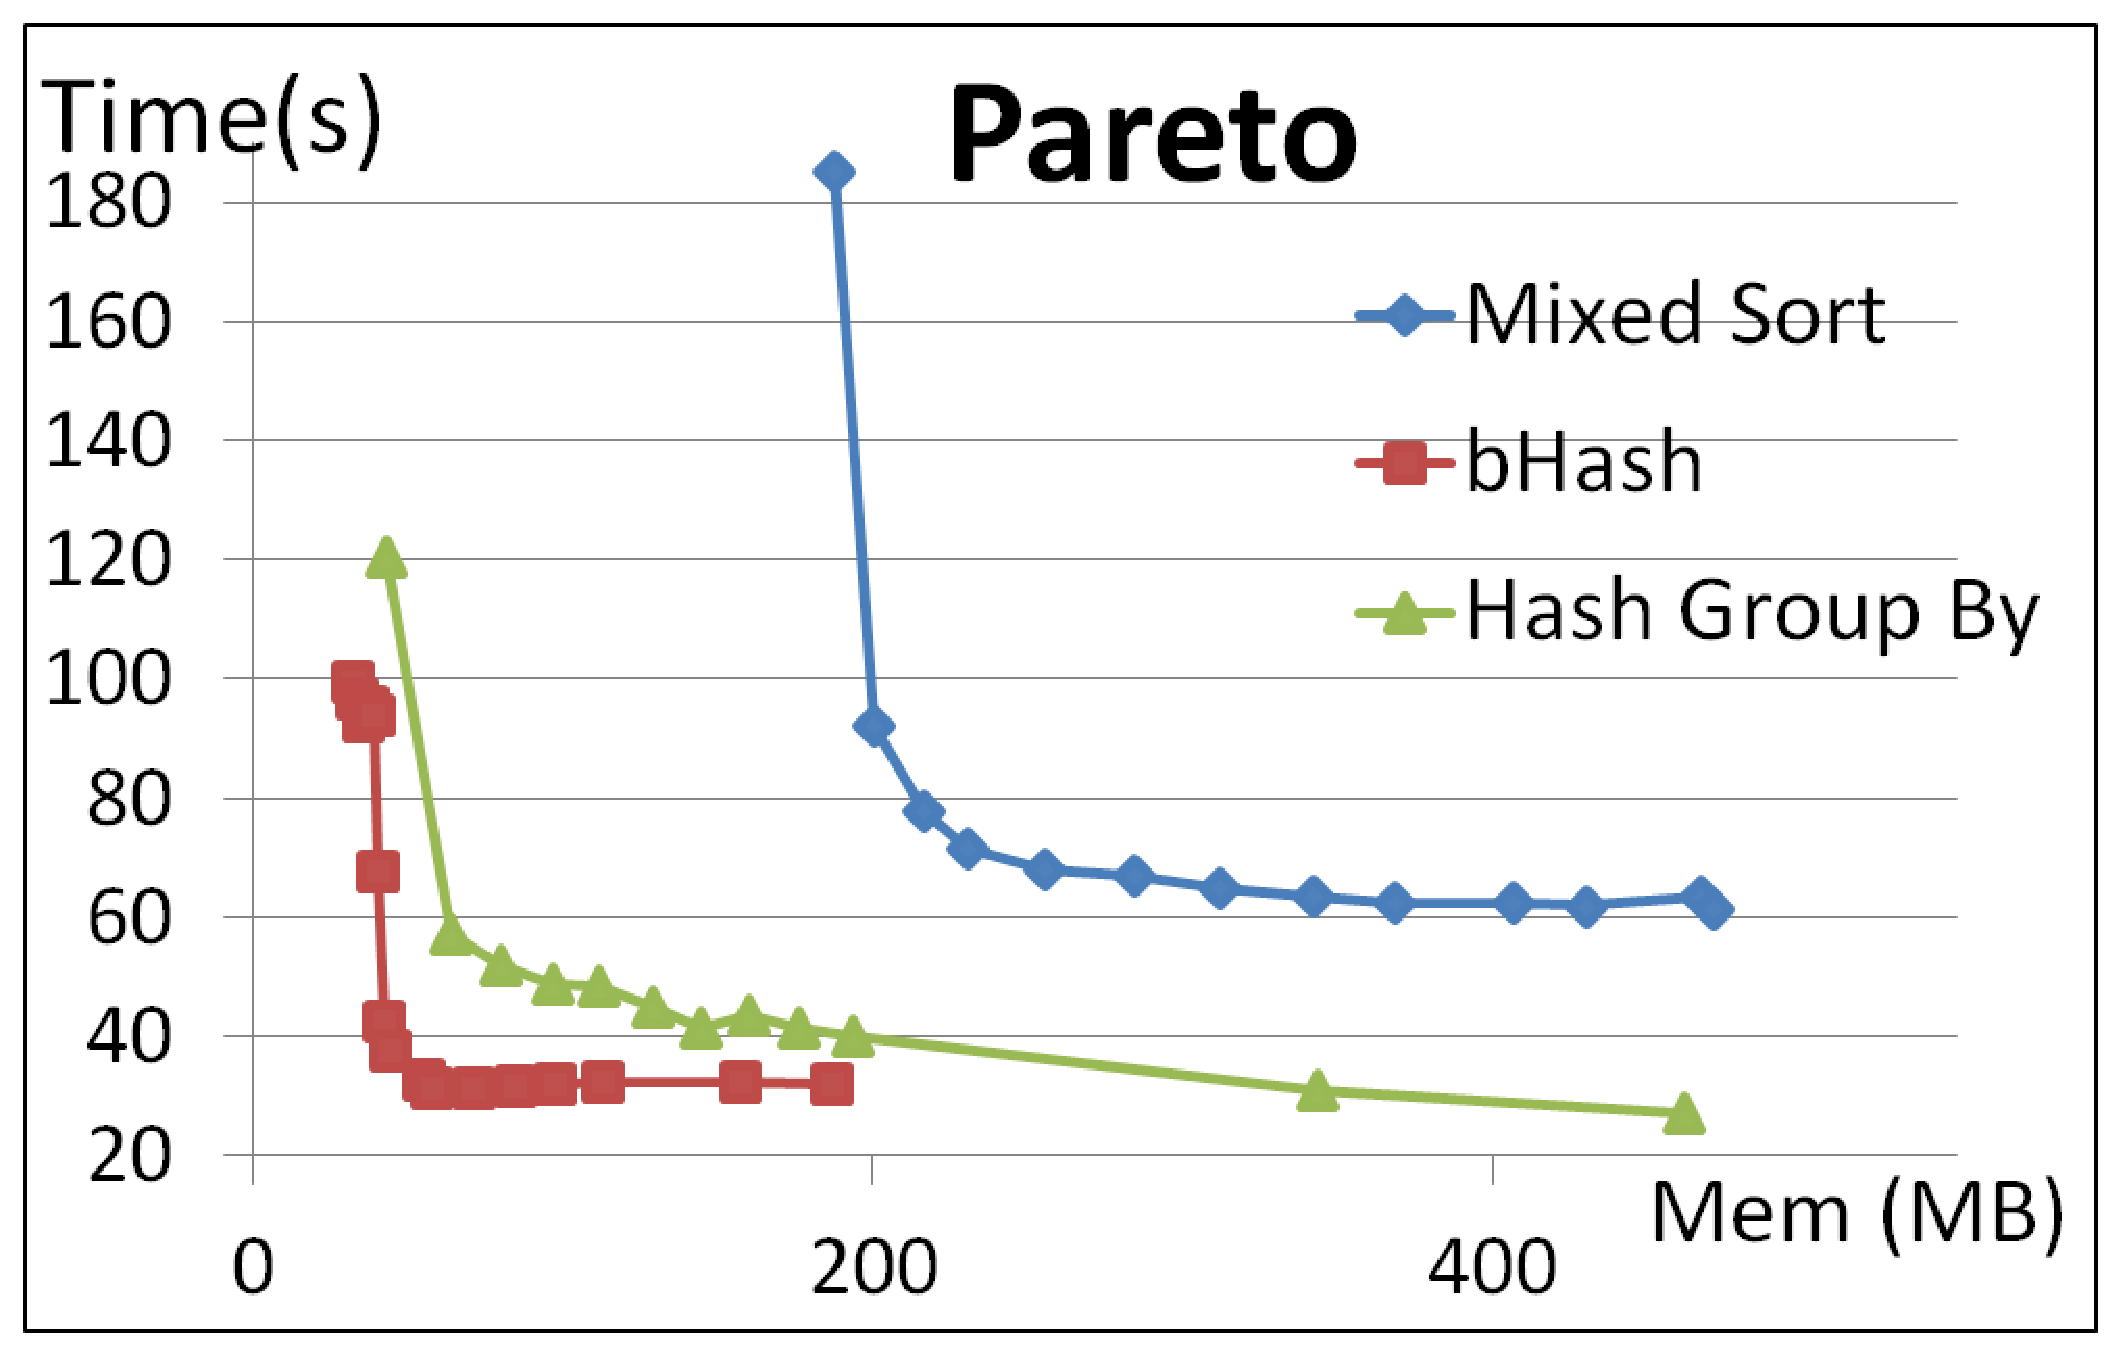
\includegraphics[width = 1.61in]{fig/paretoMemTime.eps}\label{fig:paretoMemTime}}\ \
    % \hspace{2pt}
%    \subfloat[Running time for various file numbers]{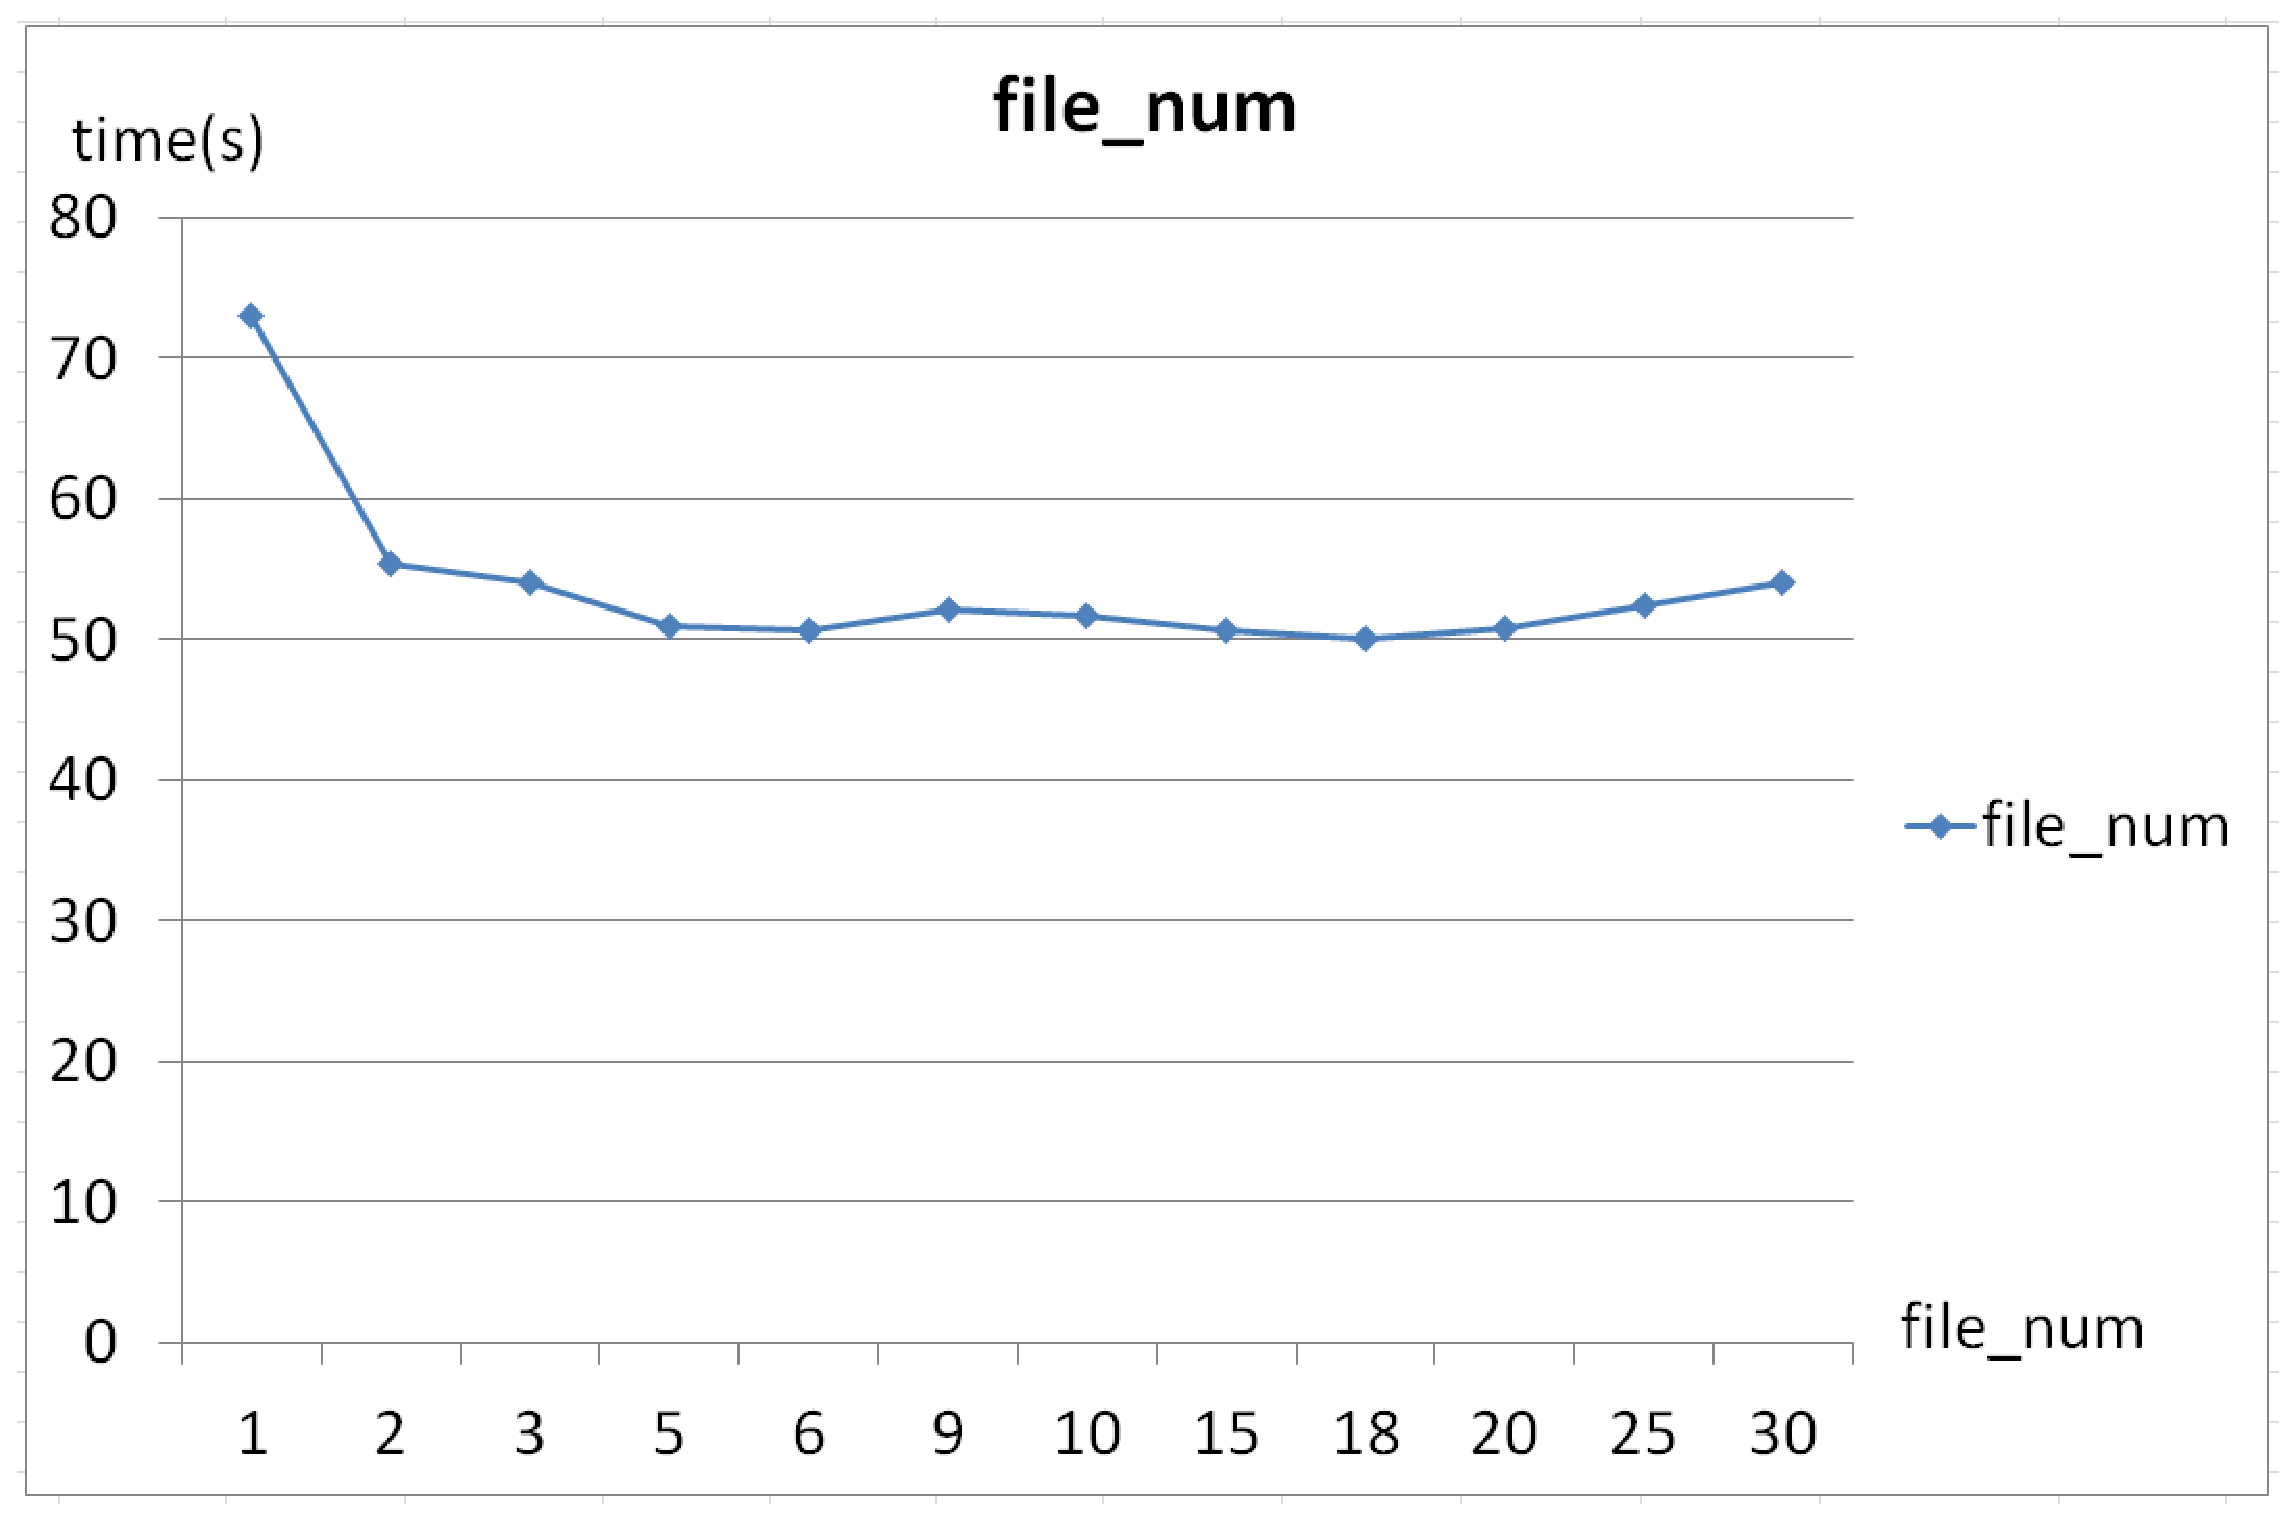
\includegraphics[width = 2in]{filenumTime.eps}\label{fig:buffersizeTime}}\ \
%     \hspace{2pt}
%    \subfloat[Memory usage for various file numbers]{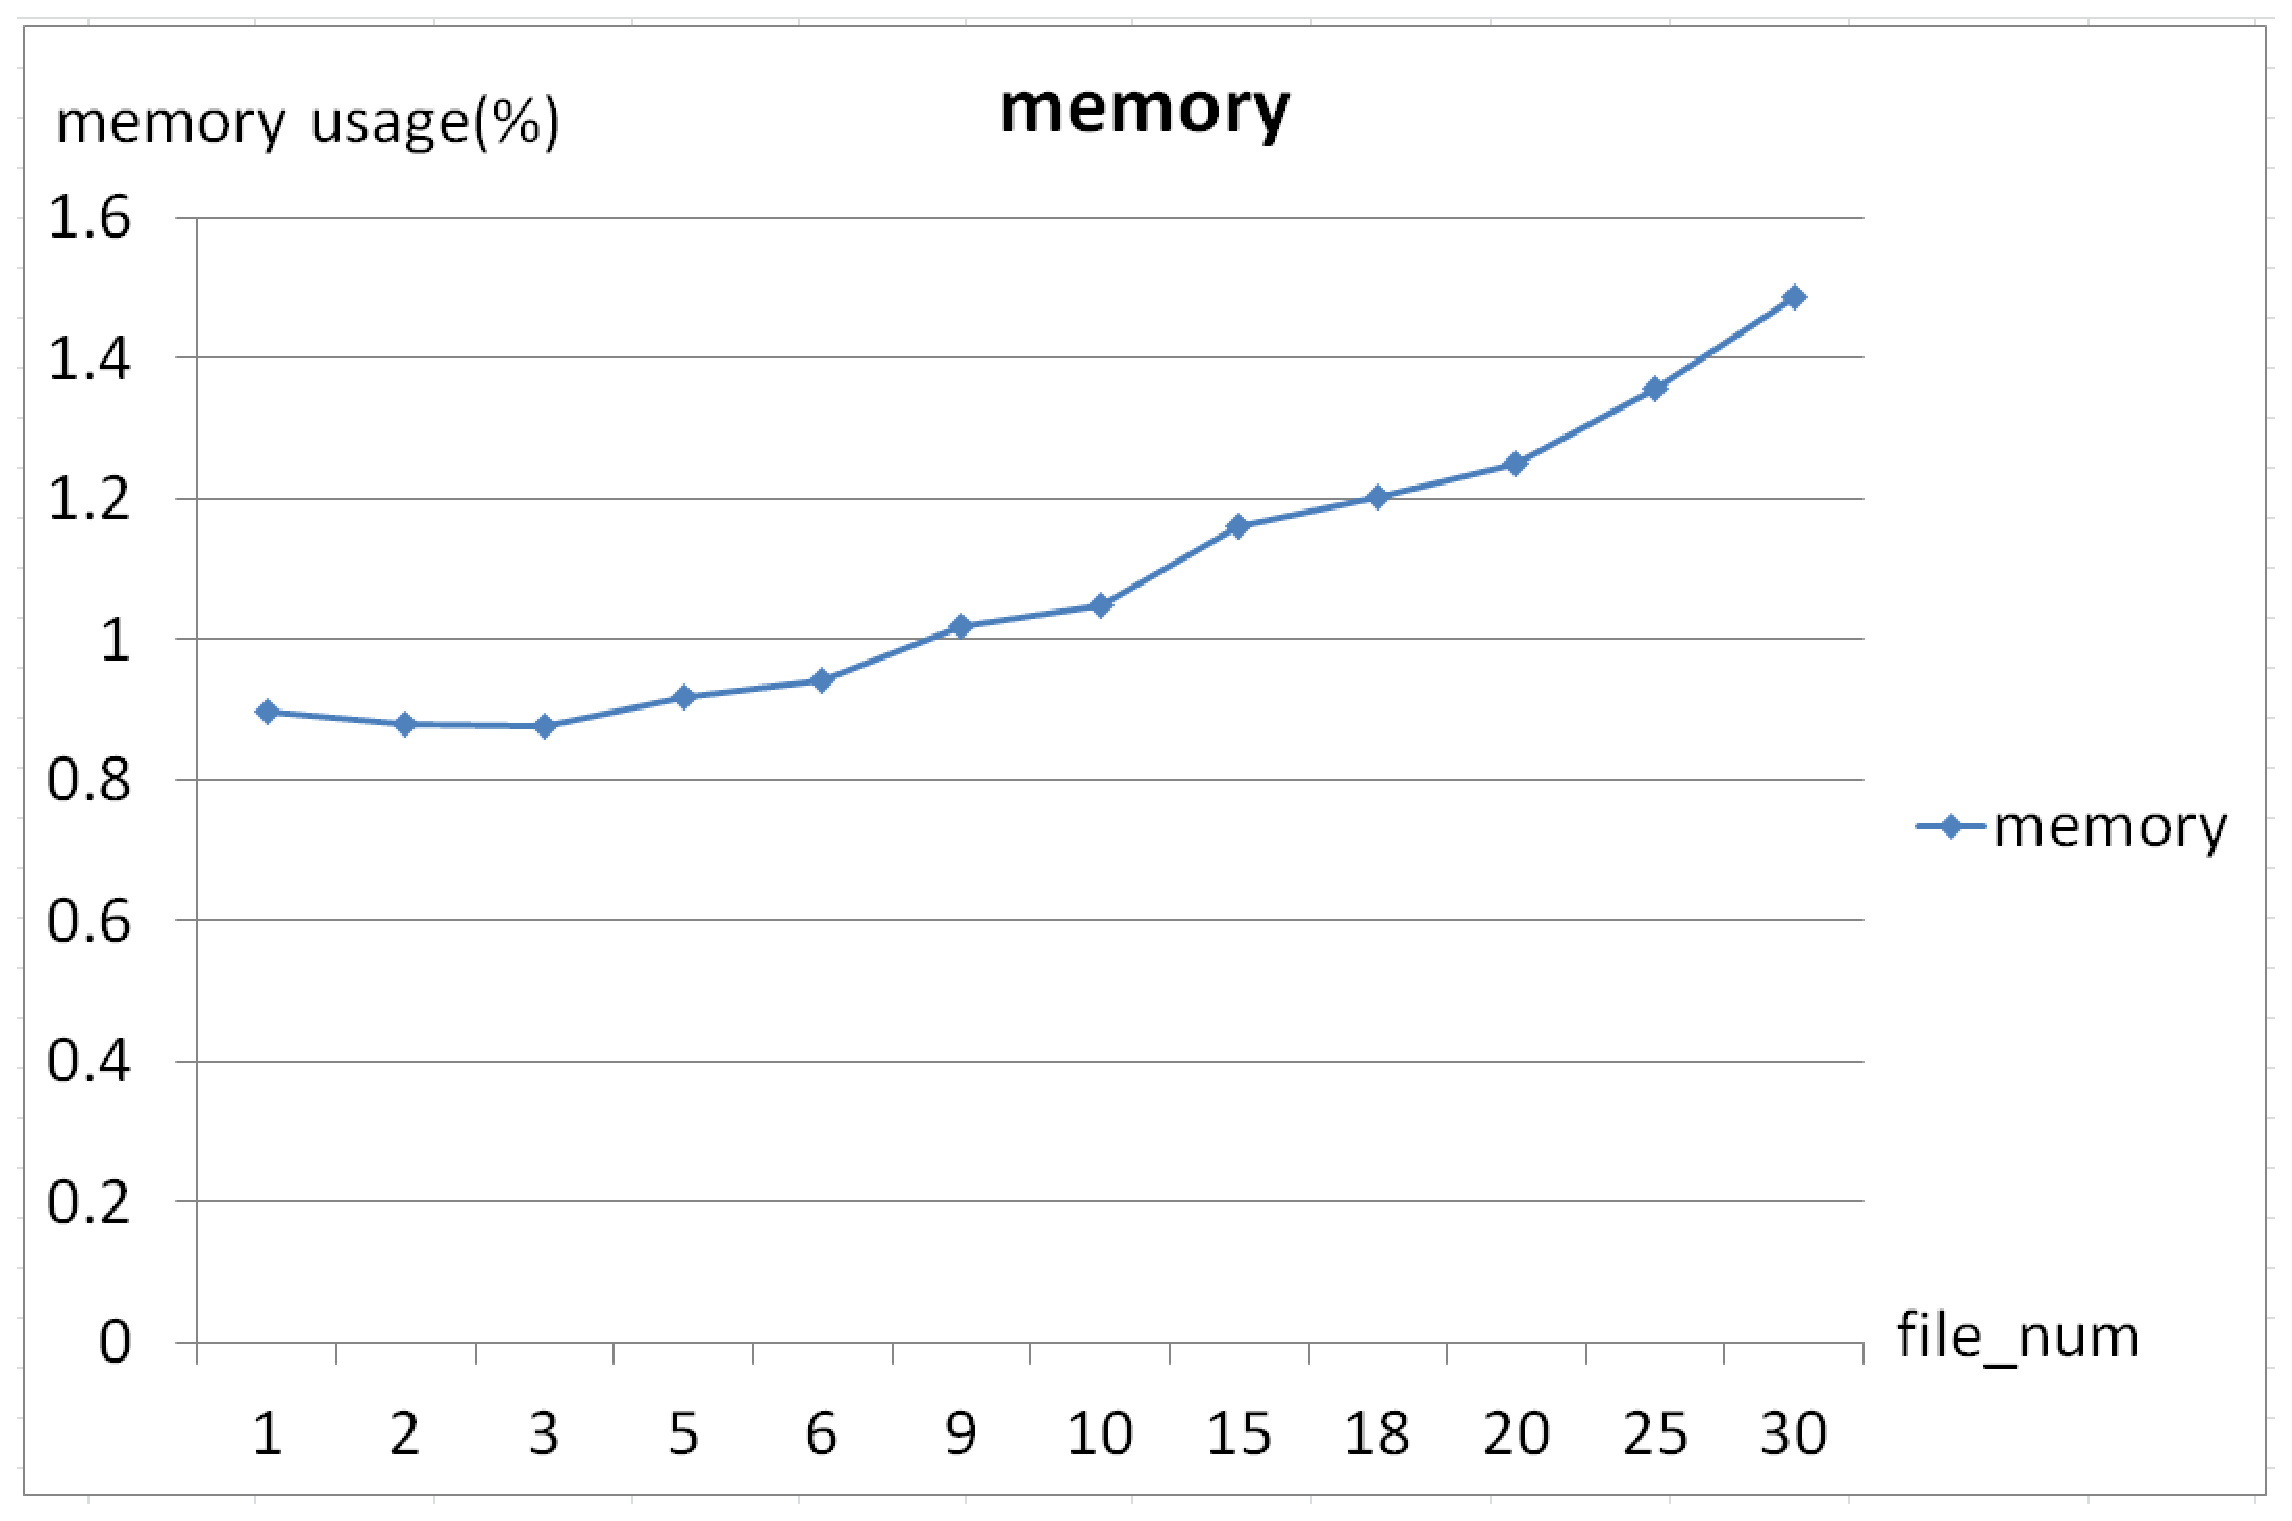
\includegraphics[width = 2in]{filenumMem.eps}\label{fig:buffersizeTime}}\ \
    \caption{Performance comparison on various data sets.}\label{fig:Performance comparison evaluation}
\end{figure*}

\begin{table}
  \caption{Data sets}
  \label{tab:commands}
  \begin{tabular}{ccl}
    \toprule
    dataset &size & illustration\\
    \midrule
    Twitter & 180.4MB& Twitter social network statistics data\\
    Google & 97.2MB & Google web graph data\\
    Wiki	&1.2GB	& Wikipedia access data in one day\\
    Normal	&589.6MB& Normal distributed simulation data\\
    Pareto & 575.4MB & Pareto distributed simulation data\\
    Gama & 594.8MB	& Gama distributed simulation data\\
    \bottomrule
  \end{tabular}
\end{table}

All serial methods were implemented in C++, and compiled with g++ version 4.8.4 in Linux. The experiments were executed on a machine with two quad-core Intel CPUs at 2.67GHz and 32GB RAM.



\subsection{Overall Performance Evaluation}

The following experiments compare bHash against merge-sort and memory-constraint hash. In order to compare these algorithms fairly, we added a buffer for each file in the merge phase of sort grouping. During evaluating the grouping time, we have allotted to all algorithms the same amount of memory. In this experiment, we also investigate the time performance of the three grouping methods with memory usage varying.

Figure 3 (a) compares the grouping time of three methods for different data sets as showed in Table 1 with the same memory size ranging from 0.2\% to 2\%. bHash is consistently faster compared to the other algorithms merge-sort and memory-constraint hash using the same amount of memory. Merge-sort algorithm is the slowest one among the three methods, because there is unnecessary computational overhead in aggregating kv-pairs with merge-sort algorithm as we have analyzed in section \uppercase\expandafter{\romannumeral2}. For the simulation data sets Normal, Pareto and Gama whose size is almost same, merge-sort costs almost the same time, which verifies the feature of no data distribution dependency (has shown in section \uppercase\expandafter{\romannumeral2}). Figure 3 (b) and (c) show the running time acceleration percentage of our bHash compared the existing algorithms: merge-sort and memory-constraint hash respectively using the same amount of memory. The experiment result shows that the processing of various data sets is at least 20\% times faster than merge-sort and even up to 57.8\% times. It speeds up the execution time compared to memory-constraint hash from 4\% to 45\%. What's more, for the long-tailed distributions such as Pareto, our algorithm even achieves 50\% better overall performance than merge-sort but occupies 40\% times less memory and 45\% faster than memory-constraint hash with 39\% times less memory.

Simulation data sets are mainly to evaluate the robustness of our algorithm for grouping data with different distributions especially for skewed data like long-tailed distributions. We generate three representative distributions data, Normal \cite{marsaglia2004evaluating}, Pareto \cite{rootzen2006multivariate} and Gama \cite{minka2002estimating}. The Normal distribution is the most popular data distribution in real world. As figure 3 shows, bHash improves the time performance up to 32.9\% compared to merge-sort and 7.7\% compared to memory-constraint hash. When the data skews seriously, the grouping performance of memory-constraint hash algorithm drops sharply. The running time comparison figure for data set Pareto and Gama shows that the execution time of memory-constraint hash algorithm is almost as much as merge-sort. In contrast to our algorithm, it improves the time performance still obviously, and is 16\% times faster than memory-constraint hash under the data set Gama. For the other data set Pareto, bHash is even 45.8\% times faster than memory-constraint hash. Therefore, memory-constraint hash is not good enough for skewed data.

We make the following analysis to this phenomenon:  Recall to section \uppercase\expandafter{\romannumeral2}, for memory-constraint hash, one or more buckets will be selected to spill to disk when the memory used has reached the threshold. Spilled partitions will be read back to re-aggregate subsequently. The long-tailed distribution makes it more difficult to divide the work data into small uniform portions. For a larger bucket spilled to disk, subsequent reading back and re-aggregating may lead to recursively execute the algorithm many times so that read and write the disk more frequently. The I/O overhead increases sharply. However, bHash performs well. As we know, the long-tailed distribution means that most of kv-pairs are distributed in a few groups. If we have fewer unique groups, the number of entries in the hash table is smaller because the algorithm keep an entry for each group and the memory required is less. Furthermore, if there are more kv-pairs mapped to the same group, the buffered kv-pairs for a group in grouping buffer will be more between two flush operation, which improves the data locality. Therefore, our algorithm is able to efficiently aggregate skewed data compared to other algorithms.

The next experiment investigates the scalability of our method. Figure 4 shows the grouping times in seconds of these algorithms with the memory available increasing. we list experimental results on some representative data sets since experimental results on other data sets are similar. On the whole, our algorithm is almost distributed lower than other algorithms in Figure 4, e.g., in the case of the same memory consumption, our algorithm performs faster and takes up less memory under the same time cost. For merge-sort and memory-constraint hash, the execution time continues to decline with the memory available increases constantly. For merge-sort, when the memory is large enough to sort kv-pairs in memory completely, the performance is no longer enhanced and memory consumption is six times than bHash(as shown in Figure 4 (b) (c) (d)). Compared to our method, memory-constraint hash need two times memory for Wiki and four times memory for Twitter to archive the same time performance. For long-tailed distributions, bHash even can save up to six times more memory compared to memory-constraint hash. For the Wiki data set, bHash curve starts on a higher memory usage as shown in Figure 4 (a), which mainly because it needs certain memory to store offset for each group. Recall to section \uppercase\expandafter{\romannumeral3}, two buffers are applied to reduce disk I/O, the buffer size is almost set to zero in the condition of the maximum execution time in Figure 4 and we increase memory consumption by increasing the buffer size in the experiment. As seen from Figure 4, bHash can achieve the best performance from the worst execution time by increasing a little more buffer. what's more, a larger memory only improves the time performance very little and waste space, which proves that our algorithm can achieve perfect performance with less memory.

In general, bHash performs from 20\% to 57.8\% times faster than merge-sort and faster than memory-constraint hash up to 45\% times in condition of using the same memory. For the long-tailed distributions such as Pareto, our algorithm even achieves 50\% better overall performance than merge-sort but occupies 40\% times less memory and 45\% faster than memory-constraint hash in the case of using 39\% times less memory. Our method can save memory up to from two to six times compared memory-constraint hash and performs well both in time performance and memory consumption.

\subsection{Parameters Evaluation}
%For these reasons using bHash, the processing of various data sets is at least 20\% times faster than Mixed Sort algorithm and even up to 57.8\% times. On the other hand, bHash speeds up the execution time compared to Hash Group By up to 45\%.

%parameterEvaluation
\begin{figure*}%figure 8
    \centering
    \subfloat[Time and memory on bucket number ]{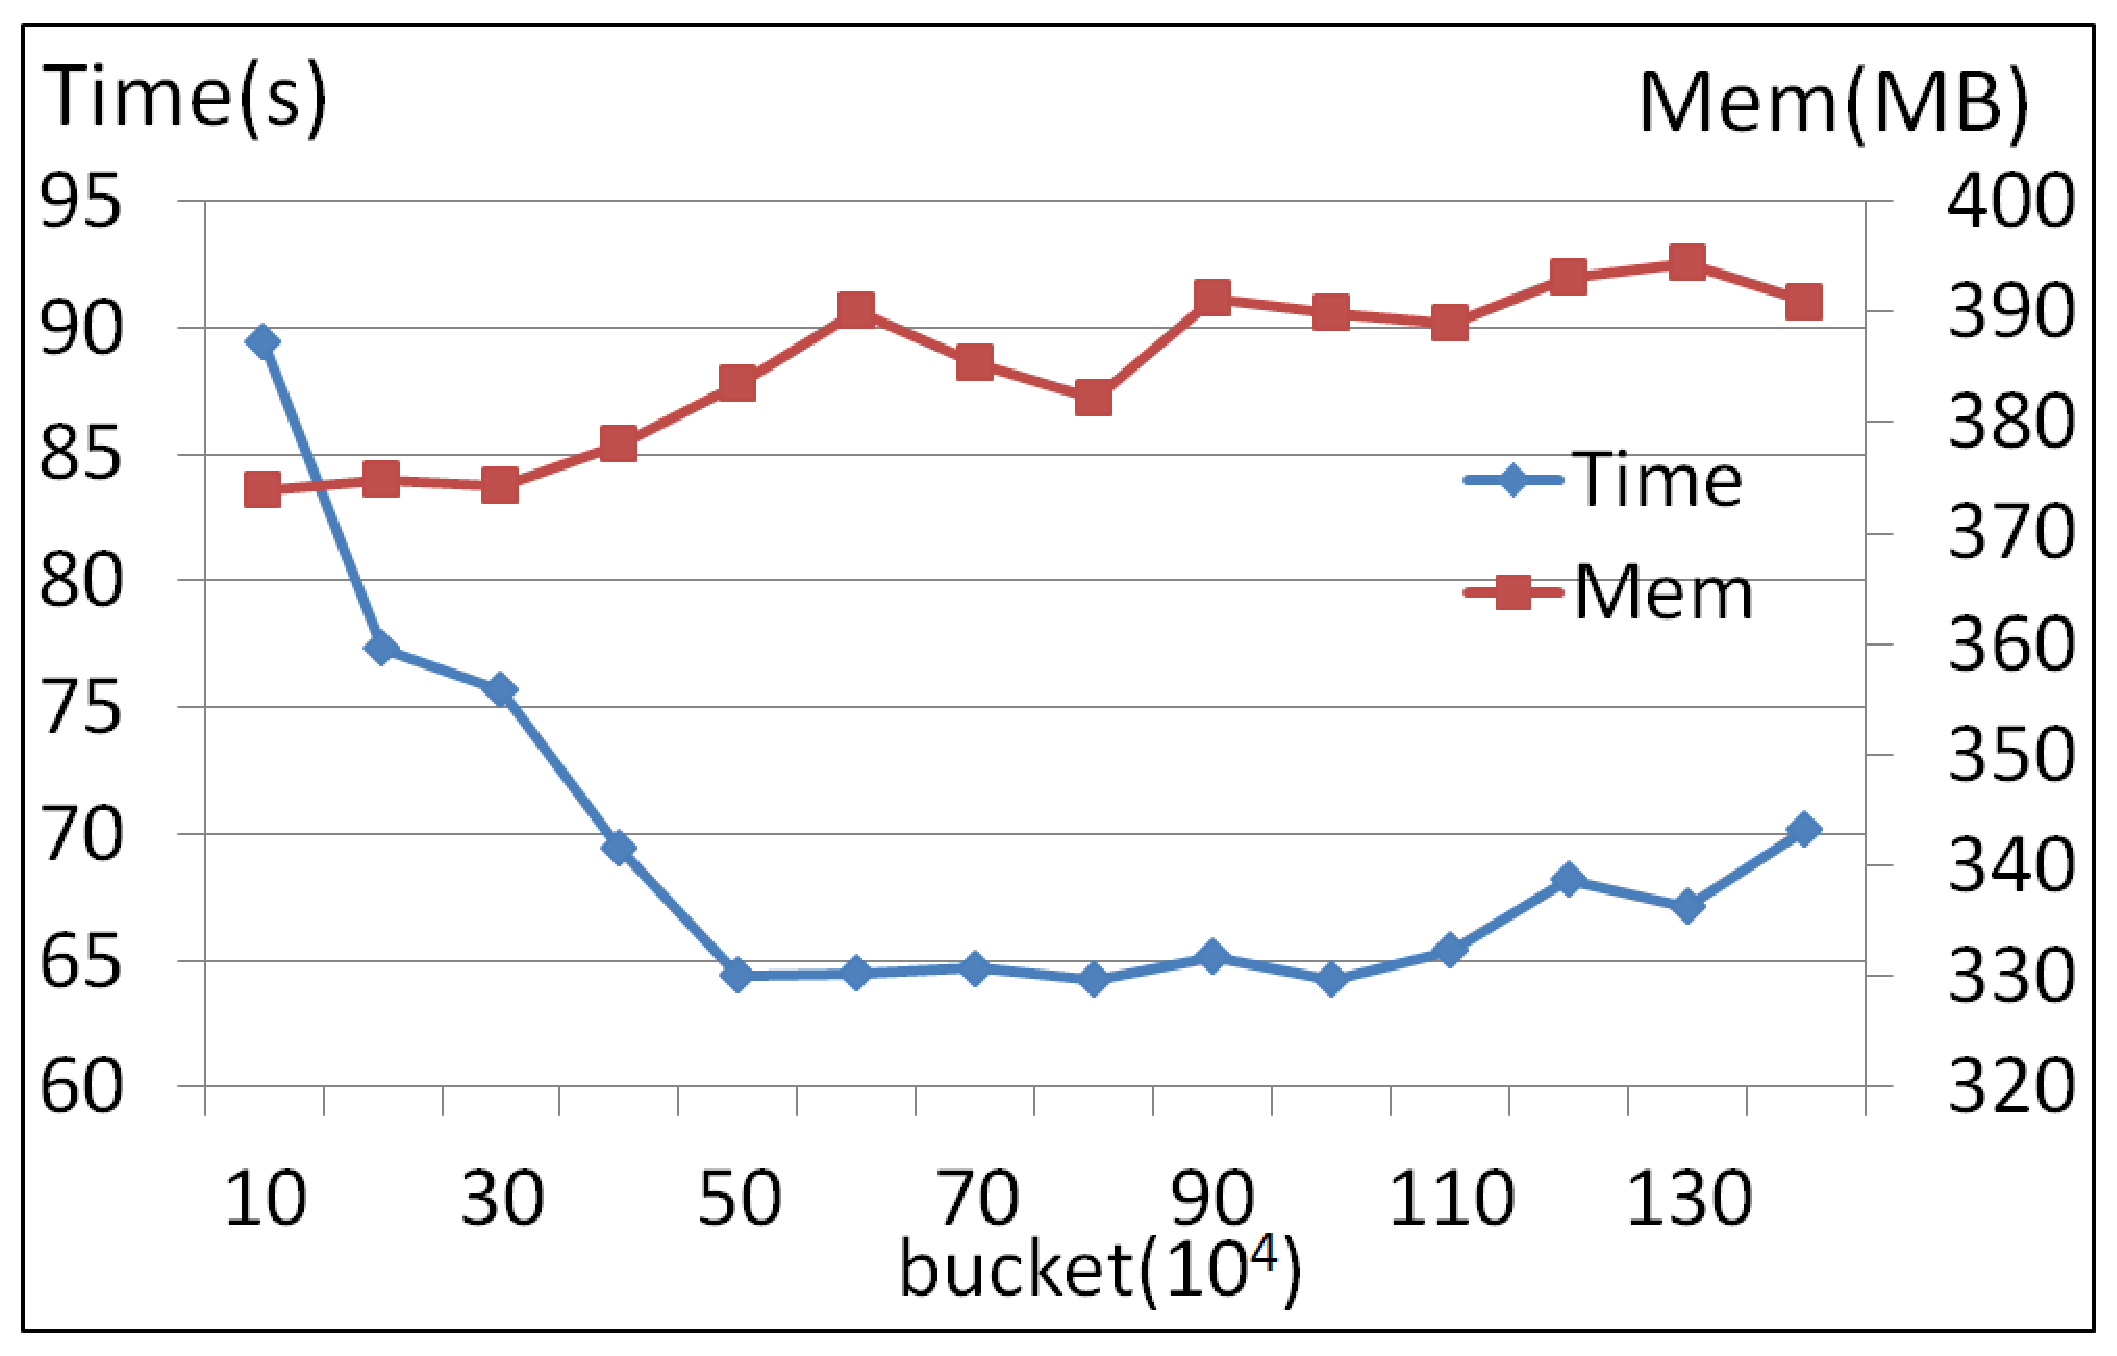
\includegraphics[width = 2in]{fig/bucketMemTime.eps}\label{fig:bucketMemTime}}\ \
    \hspace{1pt}
    \subfloat[Time and memory on grouping buffer]{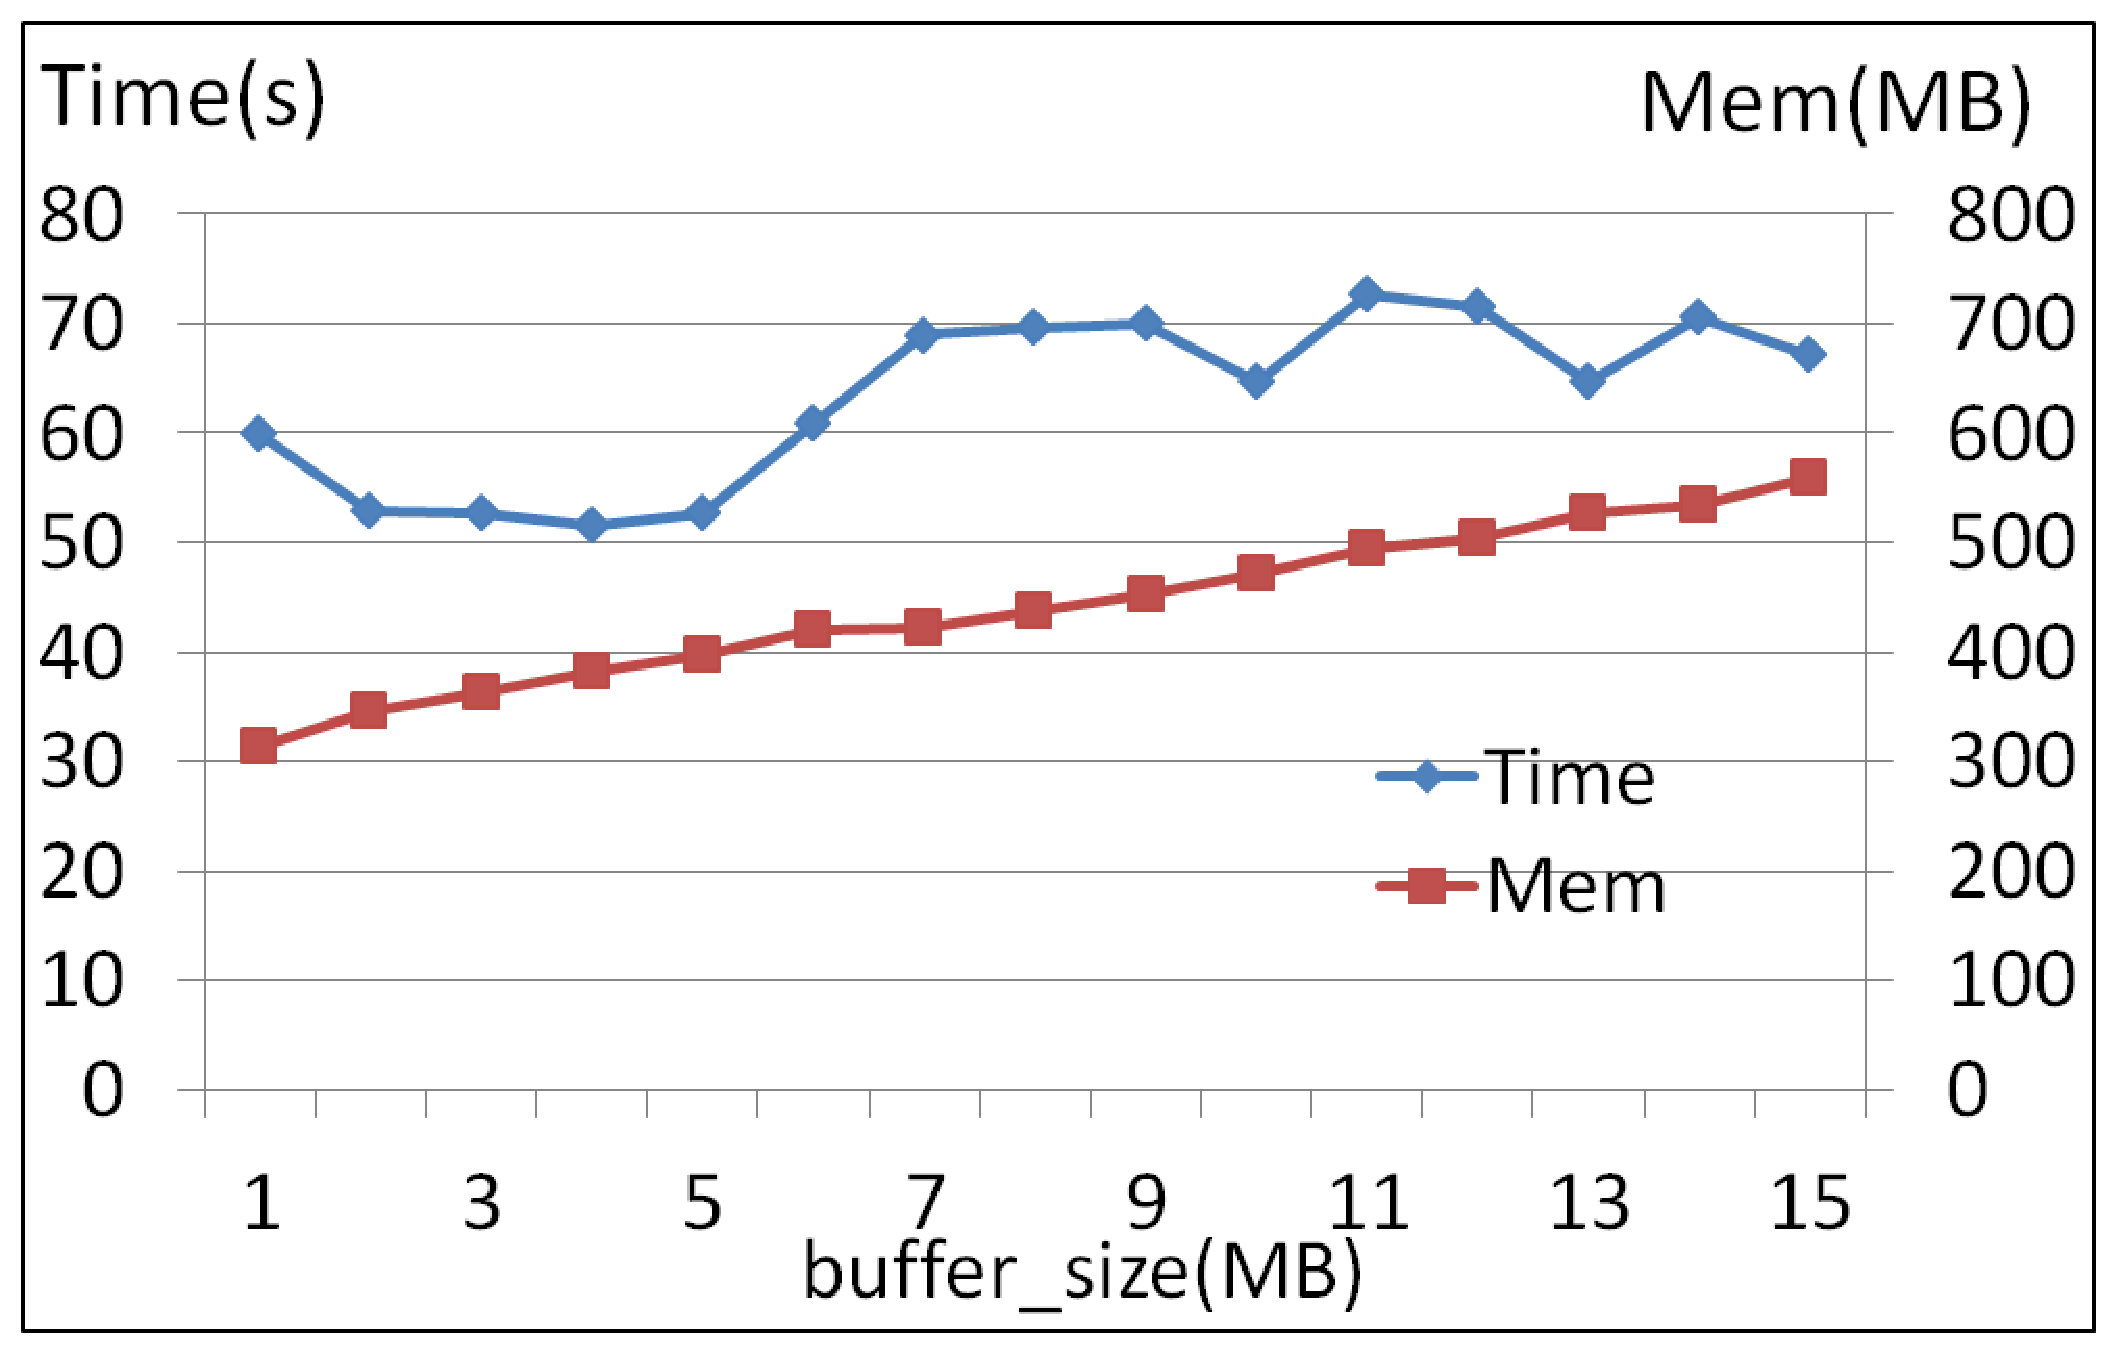
\includegraphics[width = 2in]{fig/buffersizeMemTime.eps}\label{fig:buffersizeMemTime}}\ \
    \hspace{1pt}
    \subfloat[Time and memory on sub file number]{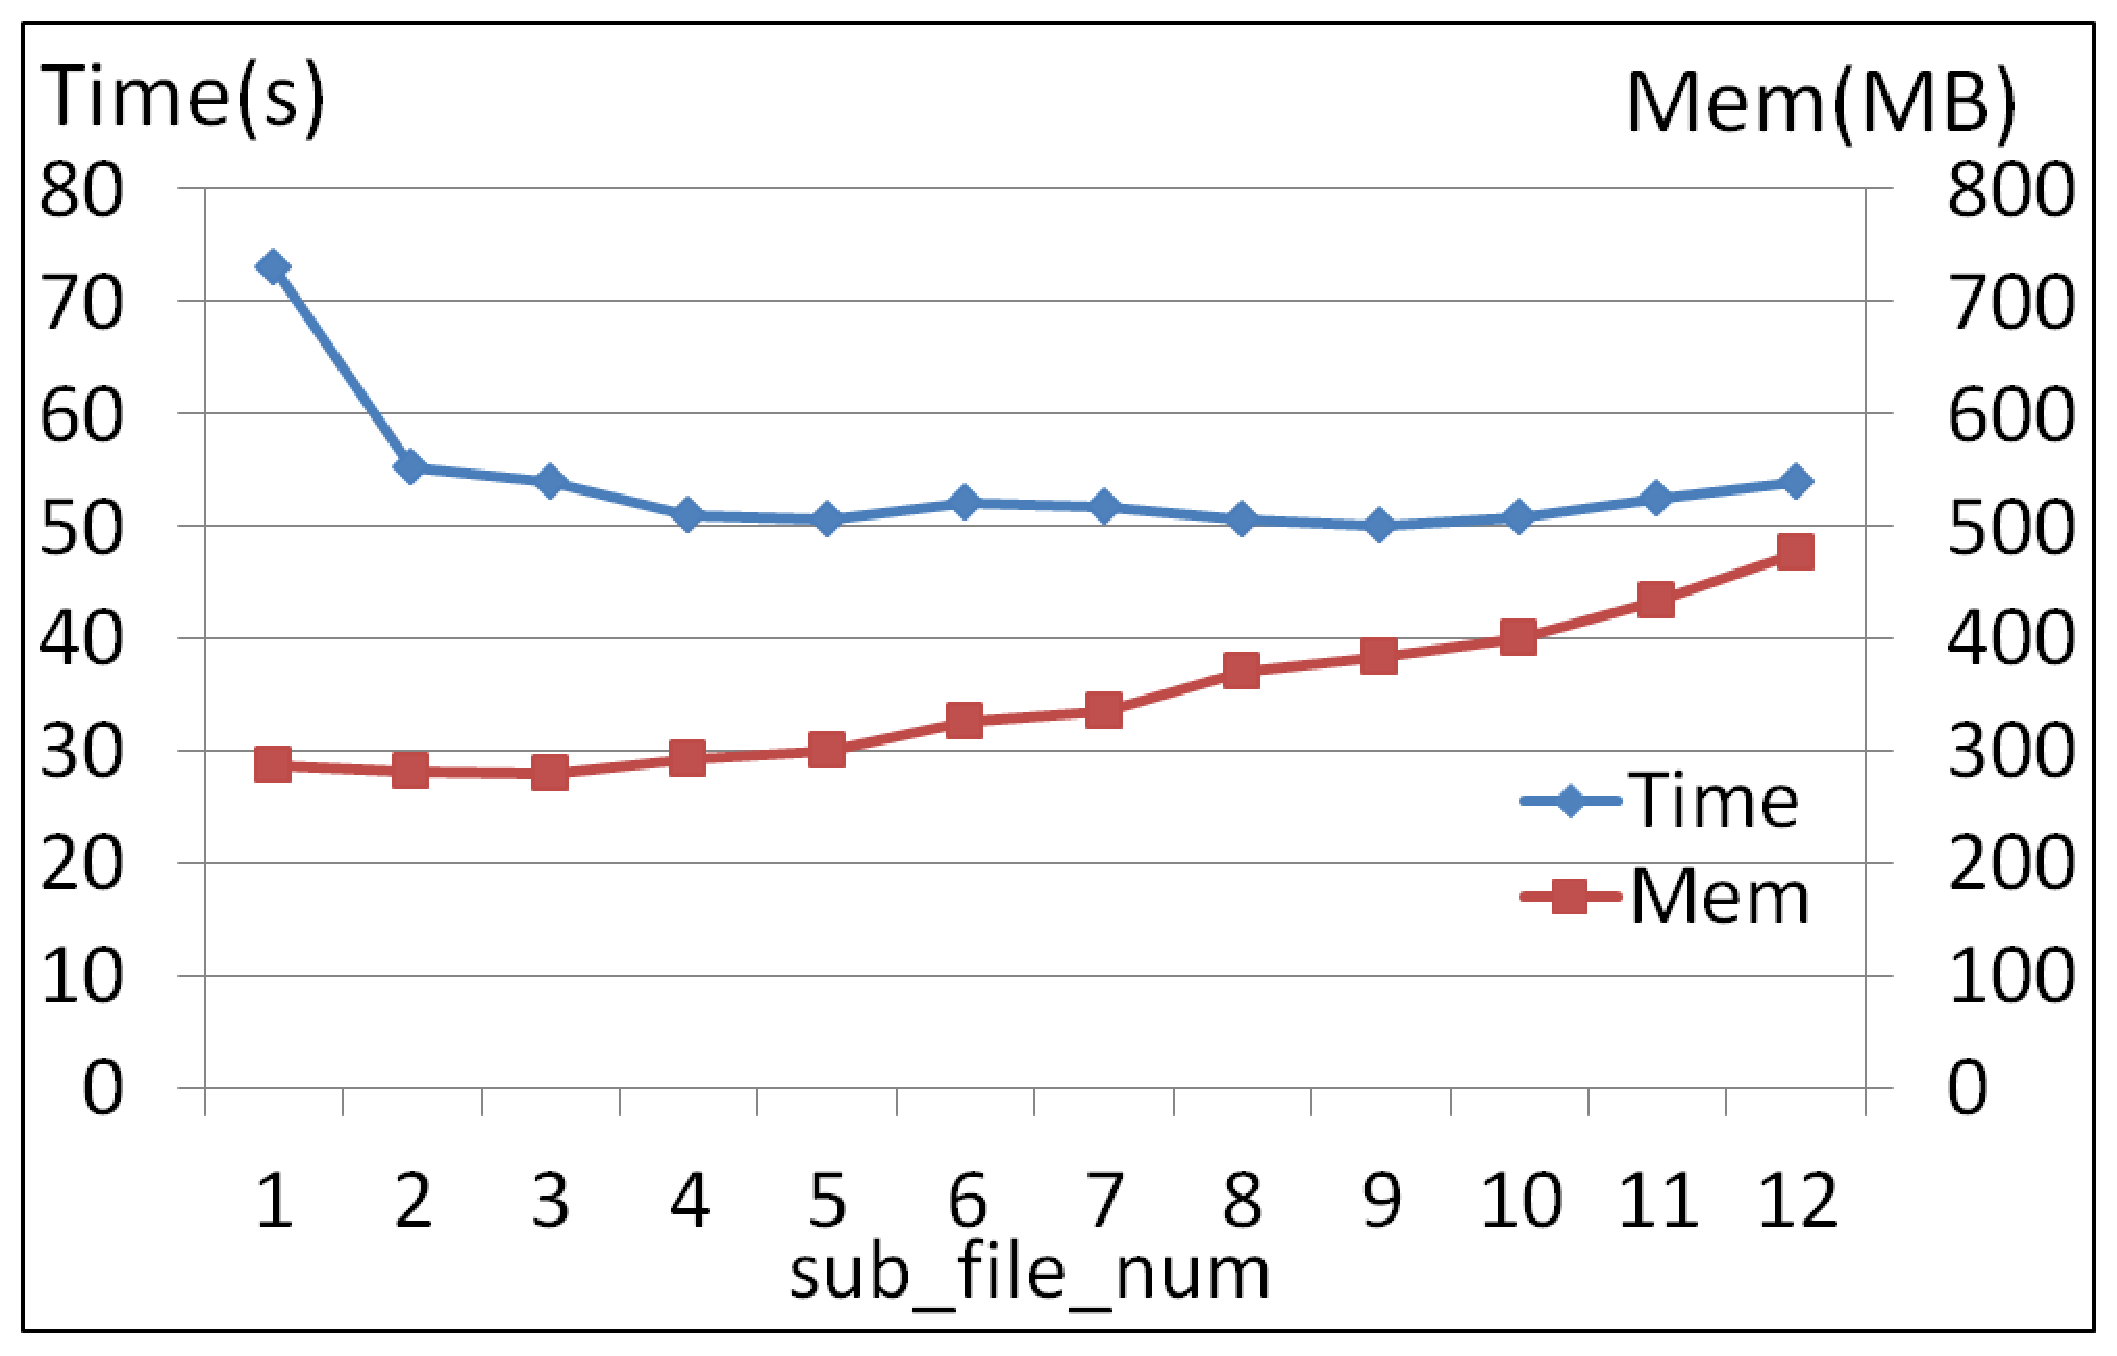
\includegraphics[width = 2in]{fig/filenumMemTime.eps}\label{fig:filenumMemTime}}\ \
    \caption{Parameters evaluation.}\label{fig:Parameters evaluation}
\end{figure*}

\begin{figure*}%figure 9
    \centering
    \subfloat[Runtime ]{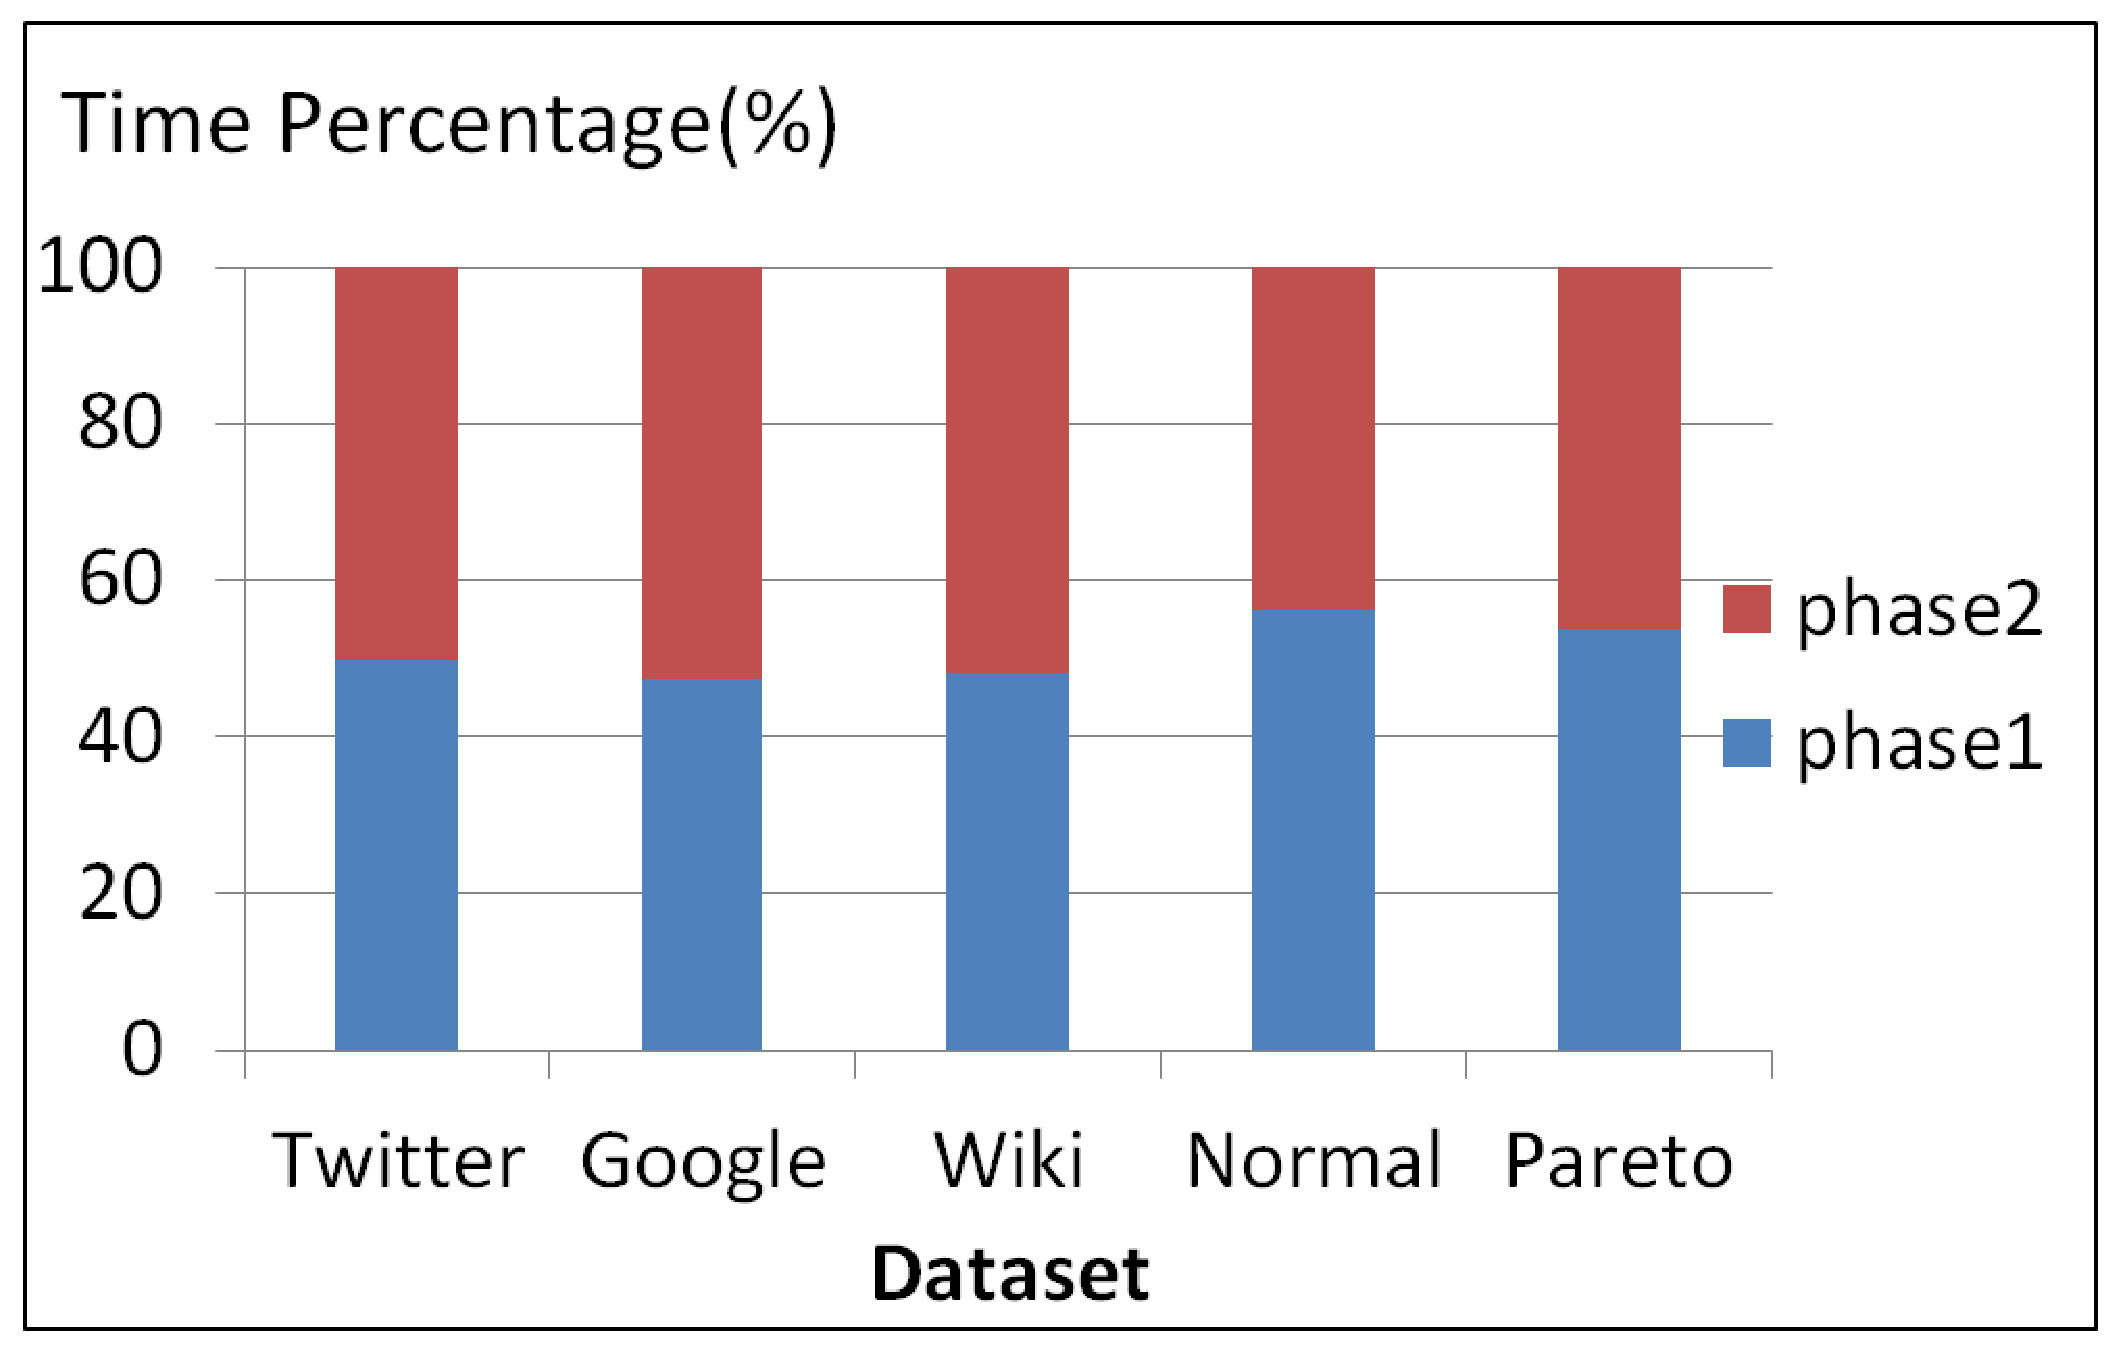
\includegraphics[width = 2in]{fig/TimePercentage.eps}\label{fig:TimePercentage}}\ \
    \hspace{1pt}
    \subfloat[Memory consumption]{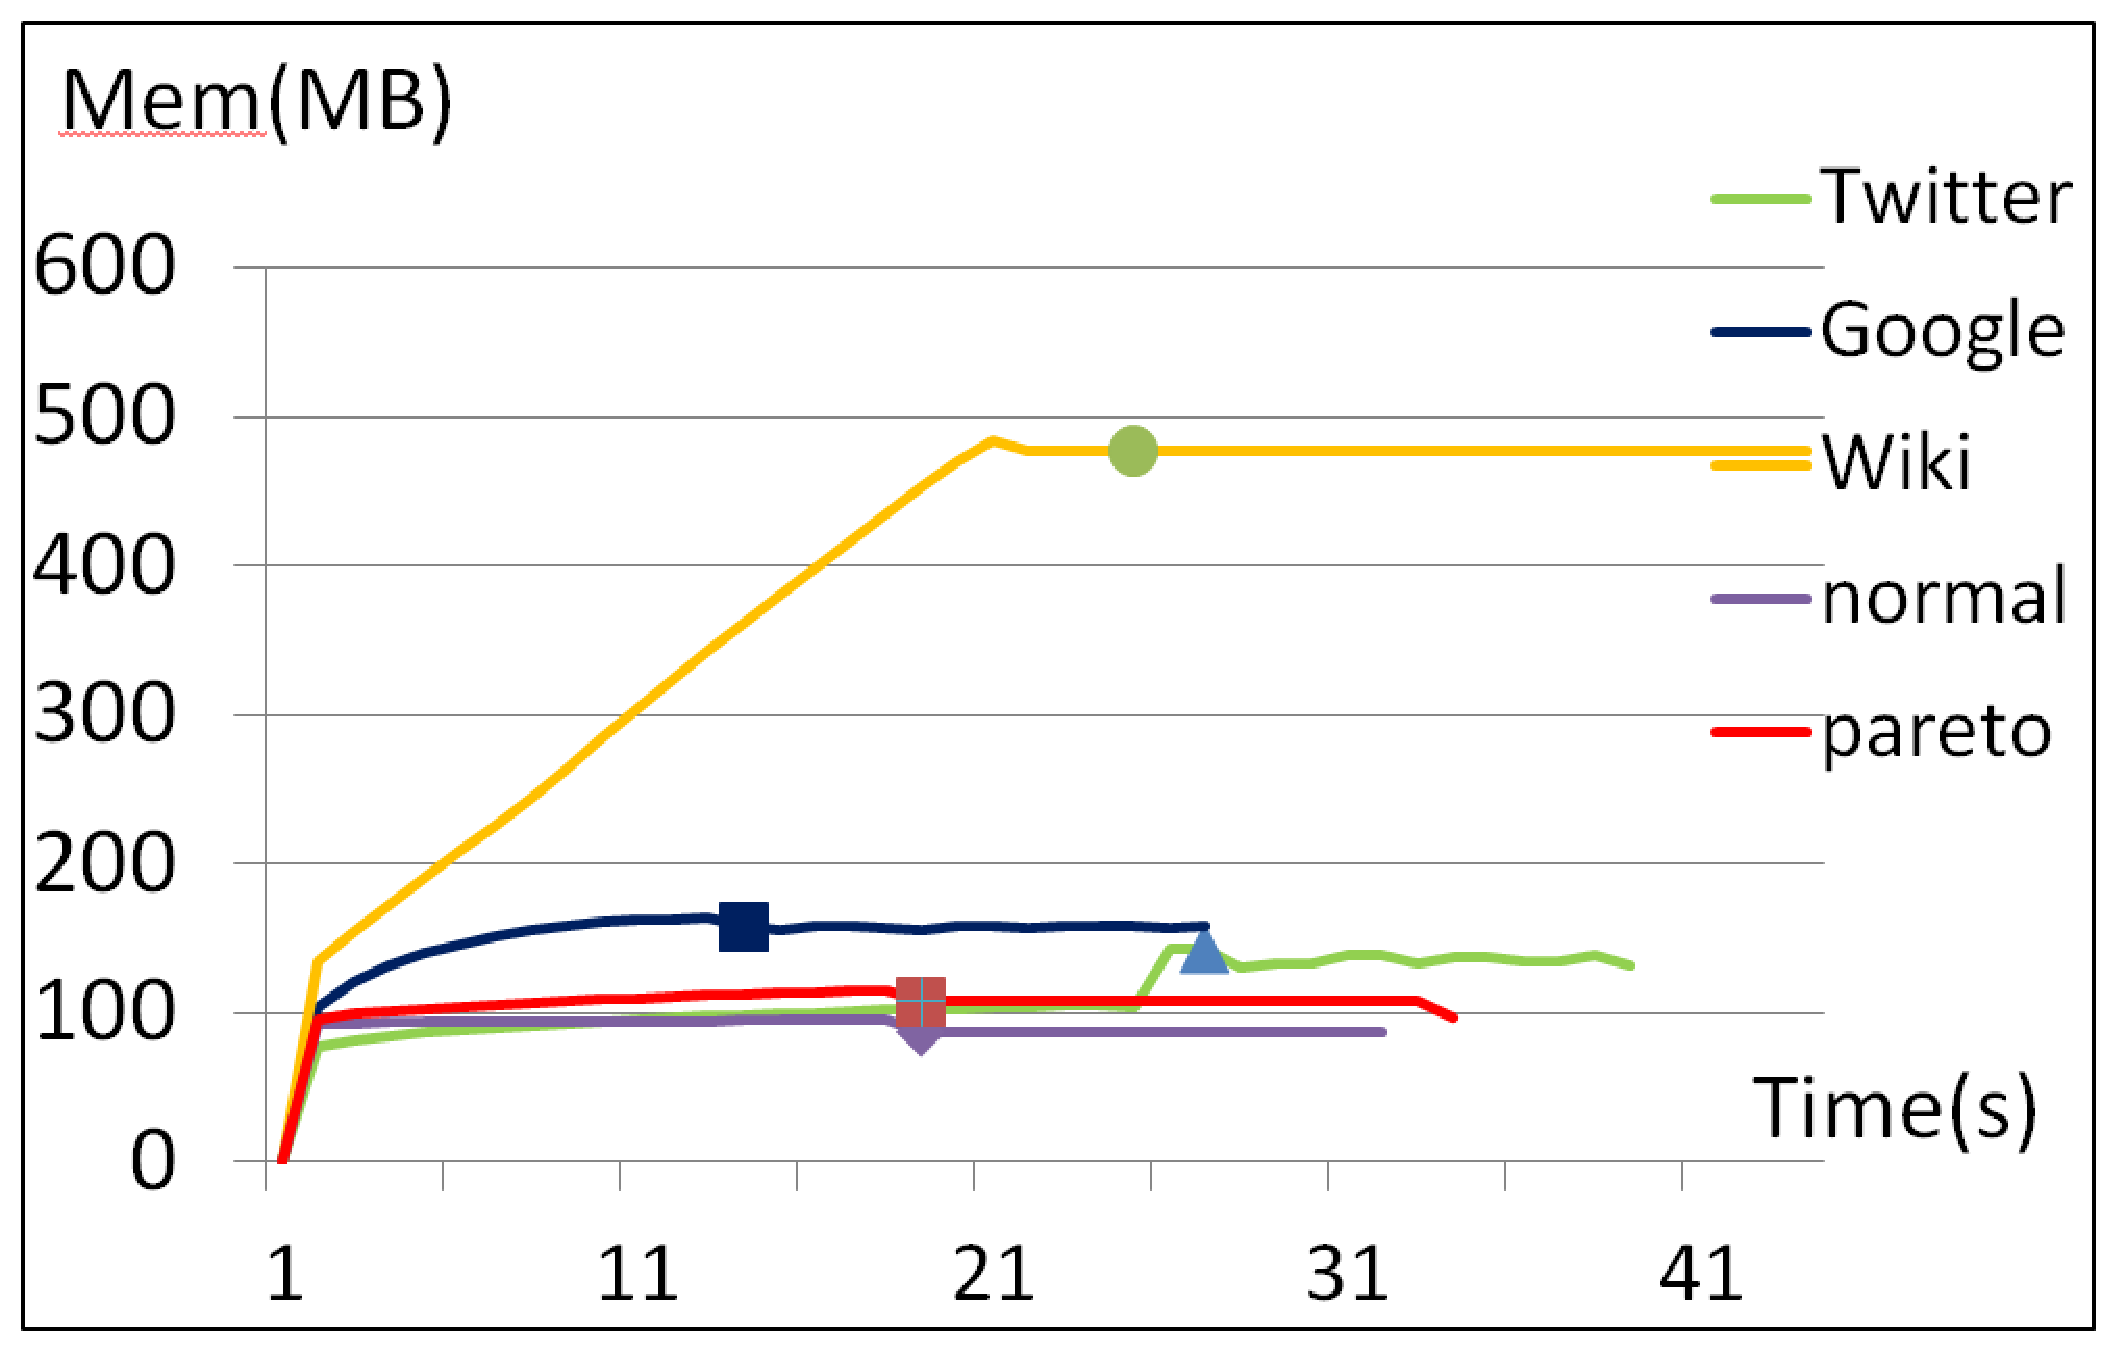
\includegraphics[width = 2in]{fig/MemPhase.eps}\label{fig:MemPhase}}\ \
    \caption{Runtime and memory consumption comparisons between two phases.}\label{fig:Phase evaluation}
\end{figure*}


In the work, we also evaluate the impact on different parameters of bHash. The number of hash buckets is set to from 500,000 to 900,000, which makes the algorithm perform best for all data sets. The number of sub files has little effect on the performance as long as greater than or equal to two. The buffer for partial grouping results is not as bigger as better. Interestingly, the execution time using a relatively smaller buffer will be shorter, which is determined by the internal mechanism of bHash. We have experimentally evaluated on various data sets in Table 1 and theoretically analyzed the effects of these parameters on the algorithm including the number of hash buckets, the size of buffer and the number of sub files. We take the representative experiment result on the maximum data set Wiki as an example. Figure 5 shows the strong scalability results for the algorithm.

\textbf{The number of buckets}. Recall from Section \uppercase\expandafter{\romannumeral3} that horizontally partitioning in bHash that splits the source file into multiple sub files to amortize the I/O cost. Figure 5 (a) compares the effect of using hash buckets of different sizes. From 100,000 to 500,000, bHash executes faster with the increase in the number of hash buckets. When the number of hash buckets is too small, one query may cost longer time because there will be more grouping entries mapped to the same bucket. In practice, the number is set to exceeding 500,000, which can archive efficient result. Too many buckets will occupy more memory as depicted in figure 5 (a). The experiment results show that the range from 500,000 to 900,000 is the best size to balance the time cost and space cost.

\textbf{Buffer size}. The next experiment shows the effect of the grouping buffer size. Recall from file filling phase in section \uppercase\expandafter{\romannumeral3} that as more grouping kv-pairs are generated, bHash uses the buffer to buffer grouping data of different groups to reduce the I/O cost because of seeking disk frequently. Figure 5 (b) compares the performance of different buffer size. Note that using a oversized buffer is not a good alternative to bHash. For example, 4M is 12\% faster than 1M for the buffer size, but it is 24\% slower than 8M for Wiki data set. Recall from the file filling in Algorithm 1, we deal with one spill at a time, the kv-pairs buffered are almost wrote to the same grouping file. If the buffer size is too large, the data buffered in buffer may involve multiple files. When one flush is triggered, kv-pairs to be flushed may belong to several files, so the seek operations will skip from a file to another file and skip back again in the next time. In order to reduce the unnecessary I/O cost, a larger buffer is not required. In our experiments, as long as the buffer size is smaller than or equals to the size of a sub file, the profits gained is the biggest no matter the time performance or the memory usage. For sub-file buffer, the effect of this parameter on performance is little and easy to understand. bHash is sufficient as long as the sub-file buffer size is set greater than or equal to fifty thousand in experiments.

\textbf{The number of sub files}. The following experiments compare the grouping time for the Wiki data set with sub file number ranging from 1 to 30 as depicted in Figure 5 (c). bHash with splitting is 24\% times faster compared to one sub file. However, when the number of sub files is larger than two, running time has not been significantly improved. Recall from Section \uppercase\expandafter{\romannumeral3}, we have allotted a buffer for each sub file to buffer the partitioned kv-pairs, thus the memory allocated continues to rise with the file number increasing as depicted in Figure 5 (c). Therefore, it is worth noting that increase the number of partition files excessively. The number of partition files is set to 10 is sufficient in all experiments.
\subsection{Phase Evaluation}
In this subsection, we discuss the impact and interrelated factor on the Statistics Collection phase and the File Filling phase. Figure \ref{fig:Phase evaluation} shows the time percentage and memory consumption on each of the two phases. Statistics collection phase studies the global knowledge of group size information and generates a offset table that contains $\langle group key, file position\rangle$s. File Filling phase writes out kv-pairs to certain file positions according to the offset table.

Figure \ref{fig:TimePercentage} shows the time percentage of the two phases on different data sets. We can notice that, for both Statistics Collection phase and File Filling phase, the time percentage is close to 50\%. Since bHash needs one pass of data in each phase and the main cost is from disk read/write, the time consumption of the two phases is almost equal.

We also compare the memory usage for the two phases on various data sets as depicted in Figure \ref{fig:MemPhase}. The mark point on each line separates the two phases and the left(right) side indicates Statistics Collection (File Filling) phase. The memory usage increases over time gradually in phase 1, which is under expected because the number of groups increases when processing more input. 


